%❖ Chương này tập trung trình bày chi tiết những gì bạn
%làm
%❖ Mô tả chi tiết phương pháp thực hiện, giải pháp đề xuất, ứng dụng phát triển
%❖ Có thể đưa ra ví dụ minh họa để dẫn nhập
%❖ Nên phân thành các mục con
%   
%❖ Hướng nghiên cứu: Phương pháp đề xuất (Proposed Approach)
%o Cơ sở lý thuyết
%o Câu hỏi nghiên cứu, giả thuyết khoa học
%o Phương pháp/Thủ tục thực hiện nghiên cứu (procedure)
%o Đối tượng nghiên cứu
%o Môi trường (phần mềm, thư viện, máy móc, công cụ, v.v...)
%o Mô tả dữ liệu, quá trình thu thập dữ liệu
%o Độ đo để đánh giá (performance metrics)

\chapter{Phương pháp đề xuất}
\label{Chapter3}

%\begin{figure}
%    \centering
%    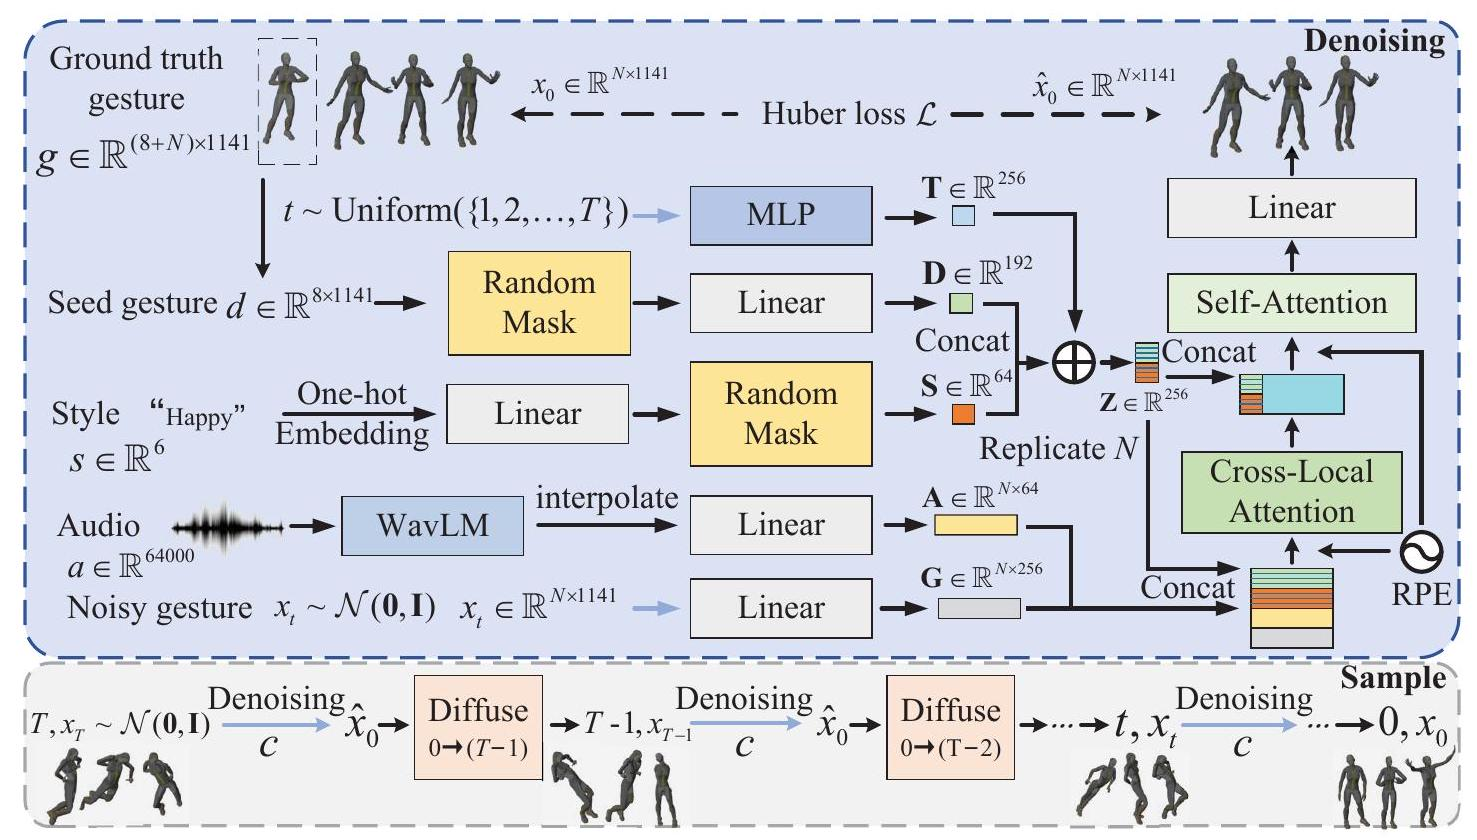
\includegraphics[width=\linewidth]{images/architecture.jpg}
%    \caption{Kiến trúc mồ hình sinh cử chỉ OHGesture}
%    \label{fig:architecture}
%\end{figure}

Trước tiên chúng tôi trình bày chúng tôi trình bày tổng quan của mô hình \ref{Overview},  và khung xương trong mỗi khung hình \ref{Skeleton} để hiểu được dữ liệu của mỗi khung hình. Từ đó chúng tôi đề xuất cách có thể trích xuất các đặc trưng về pha \ref{PeriodicAutoencoder} của mỗi khung hình để từ đó cách dùng mạng học sâu để học và điều khiển chuyển động của khung hình dựa trên pha \ref{MotionControllers}.

\section{Tổng quan mô hình}
\label{Overview}

Mô hình của chúng tôi sẽ lấy dữ liệu đầu vào ở khung hình thứ $i$ và dự đoán khung hình thứ $i+1$. Dữ liệu của mỗi khung hình là một chuỗi $\tau$ Chúng tôi sẽ trình bày 
% 

\subsection{Kiến trúc khung xương của mô hình}
\label{Skeleton}

Mỗi khung xương (skeleton) bao gồm $75$ khớp (joins) được đặt tên và minh hoạ ở hình \ref{fig:Skeleton}. 

\begin{figure}[htbp]
	\centering
	\begin{subfigure}{0.45\textwidth}
		\centering
		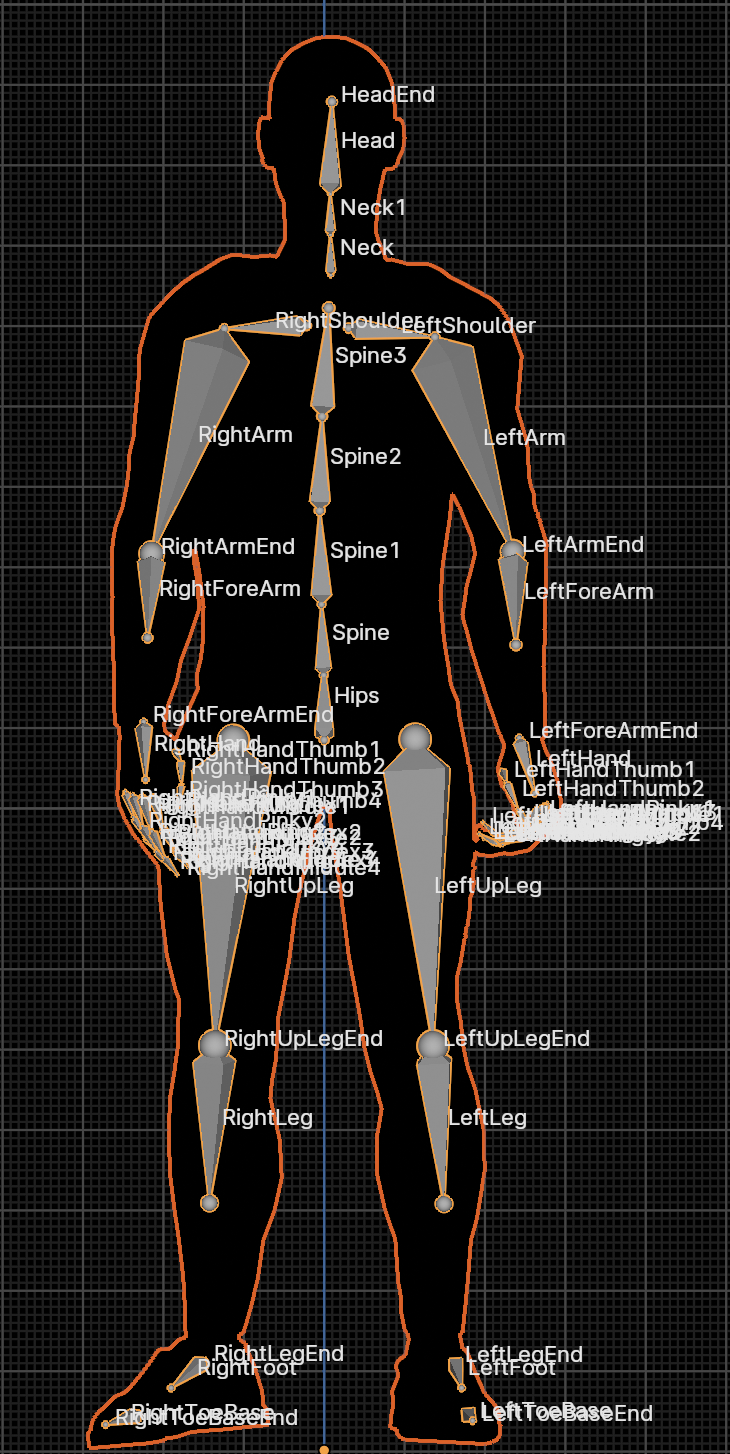
\includegraphics[height=10cm]{images/Skeleton.png}
		\caption{Khung xương và tên của các khớp của một khung xương trong mỗi khung hình.}
		\label{fig:Skeleton}
	\end{subfigure}
	\hfill
	\begin{subfigure}{0.45\textwidth}
		\centering
		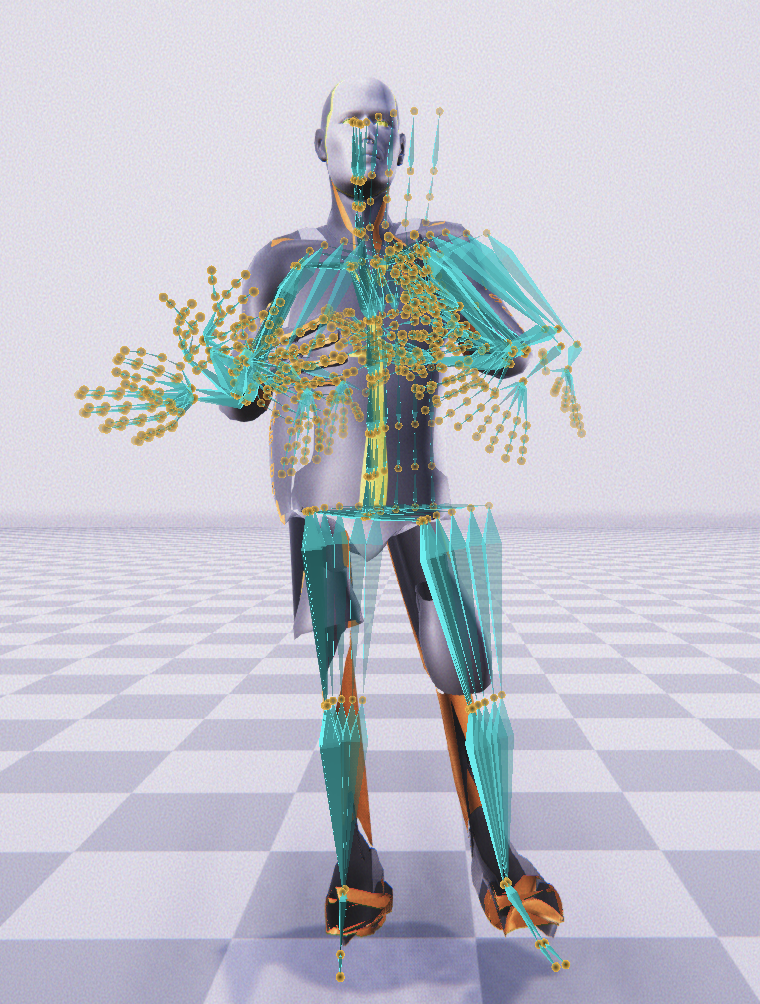
\includegraphics[height=10cm]{images/MotionPastAndFuture.png}
		\caption{Chuỗi chuyển động của cử chỉ bao gồm 6 cử chỉ quá khứ và 6 cử chỉ tương lai.}
		\label{fig:MotionPastAndFuture}
	\end{subfigure}
\end{figure}


\subsection{Đầu vào và đầu ra của mô hình}
\label{System}

%\begin{figure}
%	\centering
%	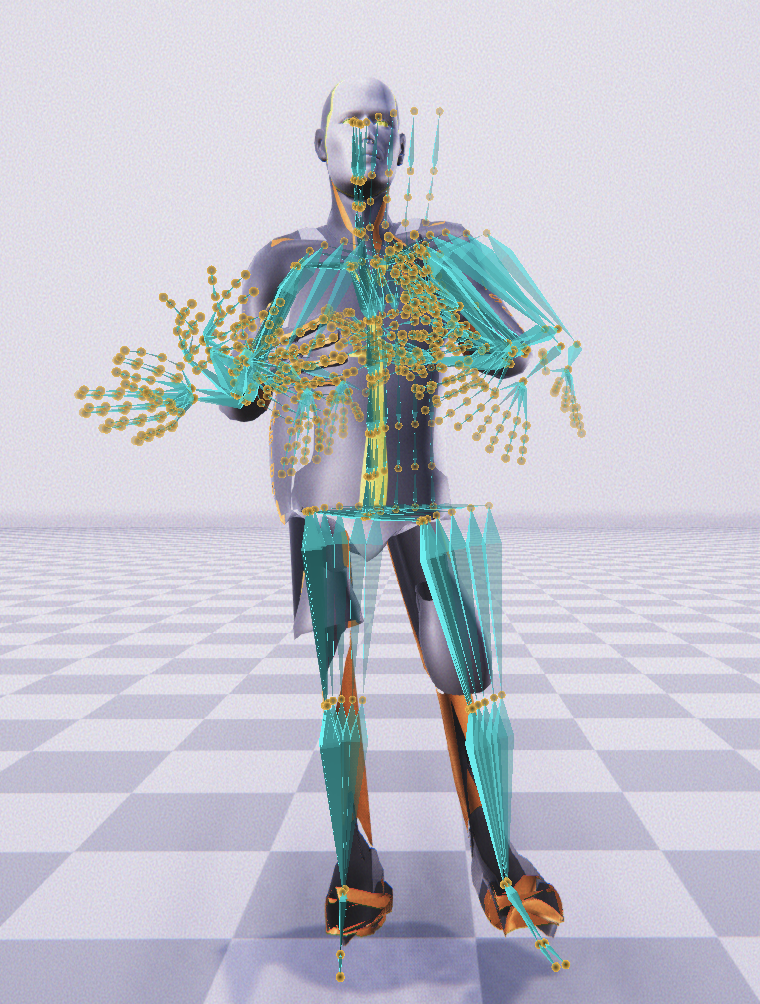
\includegraphics[height=10cm]{images/MotionPastAndFuture.png}
%	\caption{Các tham số đã học cho pha.}
%	\label{fig:MotionPastAndFuture}
%\end{figure}


\begin{figure}
	\centering
	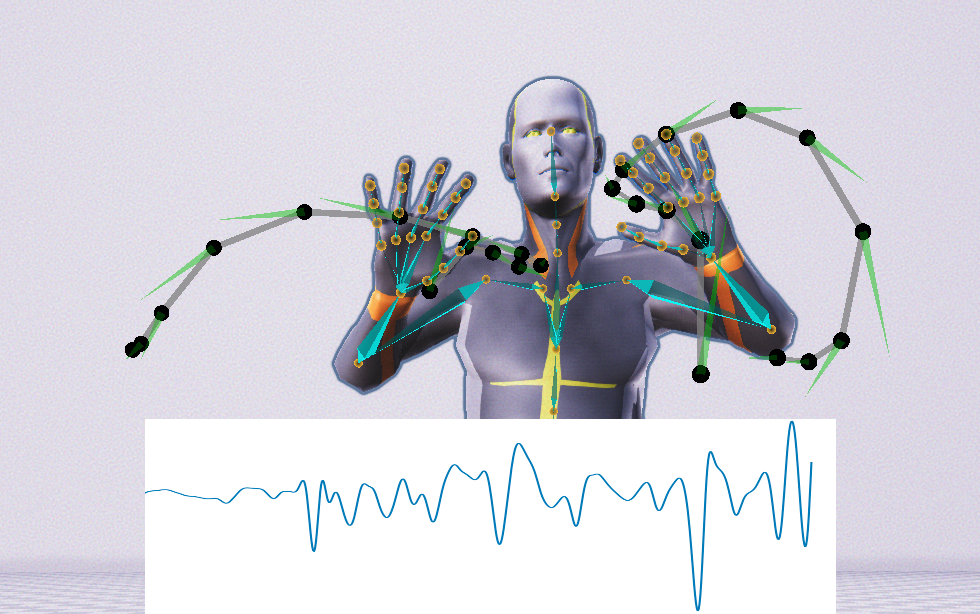
\includegraphics[height=10cm]{images/MotionSeries.png}
	\caption{Các tham số đã học.}
	\label{fig:MotionSeries}
\end{figure}

Hệ thống của chúng tôi là một mô hình chuỗi thời gian dự đoán các biến trạng thái của nhân vật, quả bóng, v.v. trong khung hình tiếp theo $i + 1$ dựa trên các biến trong khung hình hiện tại $i$. Các đầu vào và đầu ra được thiết kế sao cho hệ thống của chúng tôi có thể tạo ra các tương tác gần gũi giữa nhân vật và một đối tượng, một môi trường và một nhân vật khác. Một số biến cho điều khiển và điều kiện là hướng ứng dụng: ở đây, chúng tôi chủ yếu mô tả trong thiết lập bóng rổ, mặc dù khái niệm này là chung và có thể áp dụng cho các chuyển động khác như các thao tác của đối tượng và tương tác với môi trường. Để đào tạo, các đặc trưng Cartesian trong đầu vào và đầu ra được chuyển đổi vào hệ tọa độ gốc của nhân vật tại khung hình $i$ và $i + 1$, tương ứng. Tất cả các đặc trưng sống trong một cửa sổ chuỗi thời gian dài 1 giây, trong đó dữ liệu của 13 điểm mẫu đồng đều (6 điểm trong tương lai và 6 điểm trong quá khứ trong cửa sổ 1 giây, và một điểm cho khung hình hiện tại) được thu thập. Cách các giá trị được trích xuất từ dữ liệu ghi hình chuyển động được giải thích trong Phụ lục A.1.

\textbf{Inputs.} Vectơ đầu vào hoàn chỉnh $\textbf{X}_i$ tại khung hình $i$ bao gồm năm thành phần $\textbf{X}_i = \{ \textbf{X}^S_i, \textbf{X}^V_i, \textbf{X}^F_i, \textbf{X}^R_i, \textbf{X}^P_i \}$ trong đó mỗi thành phần được mô tả như dưới đây.

\begin{itemize}
	\item \textbf{Trạng thái Nhân vật}: \(\textbf{X}^\textbf{S}_i = \{p_i, r_i, v_i\}\) đại diện cho trạng thái của nhân vật của chúng tôi với \(B = 26\) xương tại khung hình hiện tại \(i\). Nó bao gồm các vị trí xương \(p_i \in \mathbb{R}^{3B}\), các xoay xương \(r_i \in \mathbb{R}^{6B}\) và vận tốc xương \(v_i \in \mathbb{R}^{3B}\), trong đó mỗi xoay xương được định nghĩa bằng cặp vector Cartesian tiến và lên của nó để tạo ra một không gian nội suy rõ ràng và liên tục.
	\item \textbf{Phase Chuyển Động Địa Phương} $\textbf{X}^{\mathcal{P}_i} = \Theta_i \in \mathbb{R}^{2KT}$ được đại diện bởi các vectơ pha 2D có biên độ thay đổi cho \(K = 5\) xương chính cho chân, tay và quả bóng, và được lấy mẫu dọc theo cửa sổ chuỗi thời gian từ quá khứ đến tương lai $T_{1s}^{-1s} = 13$. Các chi tiết về pha cấp xương được mô tả trong Phần 5.
	\item Third item
\end{itemize}

\textbf{Outputs} : Vector đầu ra $\textbf{Y}_i = \{ \textbf{Y}^S_i, \textbf{Y}^V_i, \textbf{Y}^F_i, \textbf{Y}^R_i, \textbf{Y}^P_i \}$ cho khung hình $i+1$

\section{Periodic Autoencoder}
\label{PeriodicAutoencoder}
%PERIODIC AUTOENCODER
	
\subsection{Network Structure}

\begin{figure}
    \centering
    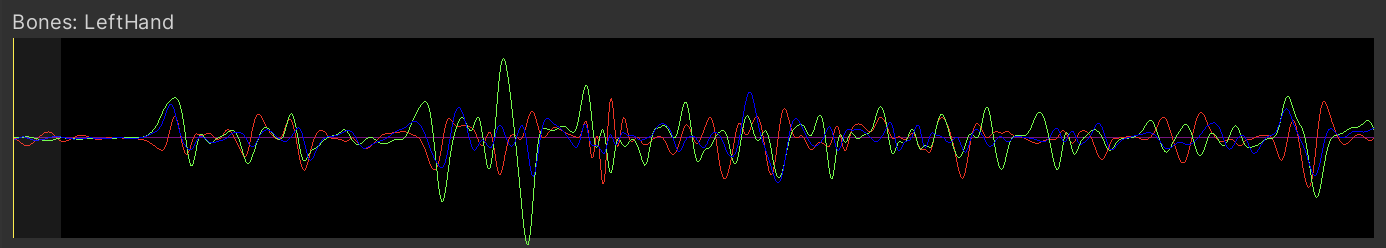
\includegraphics[width=\linewidth]{images/BoneRotationSeries.png}
    \caption{Minh hoạ sự thay đổi góc quay của một khung xương}
    \label{fig:BoneRotationSeries}
\end{figure}

Để biến đổi không gian chuyển động thành một đa tạp pha học được, chúng tôi sử dụng kiến trúc autoencoder tích chập theo thời gian tương tự như Holden và cộng sự [2015]. Tuy nhiên, ngoài việc huấn luyện mô hình để tái tạo đầu vào, chúng tôi còn bắt buộc mỗi kênh của không gian tiềm ẩn phải có dạng hàm tuần hoàn, điều này cho phép chúng tôi học một biến pha cho mỗi kênh tiềm ẩn từ một tập hợp nhỏ các tham số. Kiến trúc mạng của chúng tôi được hiển thị trong Hình 2. Dữ liệu theo thời gian được chia thành các cửa sổ chồng chéo nhau với độ dài $N$ và cửa sổ thời gian trung tâm tương ứng là $T$. Với các đường cong chuyển động đầu vào, $X \in \mathbb{R}^{D \times N}$, trong đó $D$ là số bậc tự do của cơ thể và $N$ là số khung hình của $X$, chúng tôi huấn luyện một bộ mã hóa, $g$, sử dụng các tích chập 1D để học một nhúng không gian thấp hơn của chuyển động.


\begin{equation}
	\label{eq:encoder}
	\mathbf{L} = g( \textbf{X} )
\end{equation}

Giả sử $L \in \mathbb{R}^{M \times N}$, trong đó $M$ là số kênh tiềm ẩn, tức là số kênh pha mong muốn được trích xuất từ chuyển động. Chúng tôi áp đặt tính chu kỳ bằng cách tham số hóa mỗi đường cong tiềm ẩn trong $\mathbf{L}$ dưới dạng một hàm sóng hình sin, được xác định bởi các tham số biên độ ($\mathbf{A}$), tần số ($\mathbf{F}$), độ lệch ($\mathbf{B}$) và dịch pha ($\mathbf{S}$).

Để tính toán $\mathbf{A}, \mathbf{F}, \mathbf{B} \in \mathbb{R}^{M}$, chúng tôi sử dụng một lớp Fast Fourier Transform (FFT) thực khả vi. Chúng tôi áp dụng FFT cho mỗi kênh của $\mathbf{L}$ và tạo ma trận hệ số Fourier có chỉ mục bằng không $\mathbf{c} \in \mathbb{C}^{M \times (K+1)}, K=\left\lfloor \frac{N}{2} \right\rfloor$.

\begin{equation}
	\label{eq:fft}
	\mathbf{c}=F F T(\mathbf{L}), \quad \mathbf{p}_{i, j}=\frac{2}{N}\left|\mathbf{c}_{i, j}\right|^2
\end{equation}

trong đó $i$ là chỉ số kênh và $j$ là chỉ số cho các dải tần số. Các tham số tương ứng sau đó được cho bởi


\begin{equation}
	\label{eq:PhaseExtraction}
	\mathbf{A}_i=\sqrt{\frac{2}{N} \sum_{j=1}^K \mathbf{p}_{i, j}}, \quad \mathbf{F}_i=\frac{\sum_{j=1}^K\left(\mathbf{f}_j \cdot \mathbf{p}_{i, j}\right)}{\sum_{j=1}^K \mathbf{p}_{i, j}}, \quad \mathbf{B}_i=\frac{\mathbf{c}_{i, 0}}{N}
\end{equation}

trong đó $\textbf{f} = (0, \frac{1}{T}, \frac{2}{T}, \dots, \frac{K}{T})$ là một vector các tần số. Các phép toán này cung cấp các tham số hình dạng để xây dựng $M$ hàm tuần hoàn trong khoảng thời gian, nhưng chưa bao gồm yếu tố thời gian, tức là các dịch pha của các hàm này. Để có được tham số thời gian này, chúng tôi học một lớp fully-connected (FC) riêng biệt cho mỗi đường cong tiềm ẩn, lớp này chỉ dự đoán dịch pha có dấu $\textbf{S} \in \mathbb{R}^{M}$ tại khung trung tâm của $T$ thông qua một vector trung gian hai chiều:

\begin{equation}
	\label{eq:OffsetExtraction}
	\left(s_x, s_y\right)=F C\left(\mathrm{~L}_i\right), \quad \mathrm{S}_i=\operatorname{atan} 2\left(s_y, s_x\right)
\end{equation}

trong đó $i$ là chỉ số kênh.

Từ các tham số đã học được $F$, $A$, $B$ và $S$, cùng với khoảng thời gian $T$ đã biết, ta có thể tái tạo không gian tiềm ẩn được tham số hóa $\hat{L}$ dưới dạng nhiều hàm tuần hoàn có cùng dạng kích thước như không gian tiềm ẩn ban đầu bằng cách sử dụng hàm tham số hóa $f$:

\begin{equation}
	\label{eq:Sinusoidal}
	\hat{\mathbf{L}}=f(\mathcal{T} ; \mathbf{A}, \mathbf{F}, \mathbf{B}, \mathbf{S})=\mathbf{A} \cdot \sin (2 \pi \cdot(\mathbf{F} \cdot \mathcal{T}-\mathbf{S}))+\mathbf{B}
\end{equation}


Cuối cùng, mạng giải mã không gian tiềm ẩn đã được tham số hóa bằng các phép deconvolution 1D trong bộ giải mã $h$, để ánh xạ trở lại các đường cong chuyển động đầu vào ban đầu:

\begin{equation}
	\label{eq:Decoder}
	\textbf{Y} = h(\hat{\textbf{L}})
\end{equation}

Mạng được huấn luyện bằng hàm mất mát tái tạo giữa các đường cong chuyển động gốc và dự đoán:

\begin{equation}
	\label{eq:LossFunction}
	\mathcal{L} = \text{MSE}(\textbf{X}, \textbf{Y})
\end{equation}

Điều này buộc mạng phải học sự căn chỉnh thời gian của các tư thế trên các đoạn clip chuyển động khác nhau và gán một pha thay đổi cho mỗi khung hình mới của chuyển động theo một hướng nhất định. Để thấy điều này, hãy xem xét một đoạn chuyển động có khung trung tâm tại thời điểm $t$, được trích xuất từ một đoạn clip chuyển động dài hơn và được mã hóa để tạo ra $\hat{\textbf{L}}$. Các tham số $\textbf{A}$, $\textbf{F}$ và $\textbf{B}$ giới hạn hình dạng của các tín hiệu tuần hoàn và mạng phải học cách định vị các đường cong chính xác bằng $\textbf{S}$. Đối với một đoạn chuyển động có khung trung tâm tại thời điểm $t + 1$, được trích xuất từ cùng một đoạn clip chuyển động, chúng ta kỳ vọng rằng mọi thay đổi trong $\textbf{A}$, $\textbf{F}$ và $\textbf{B}$ sẽ rất nhỏ (xem Hình 3), vì vậy $\textbf{S}$ cần phải tiến triển để giữ cho không gian tiềm ẩn đồng bộ với chuyển động, vì cùng một bộ giải mã tích chập được sử dụng. Điều này có nghĩa là mô hình phải học cách dự đoán các vector 2D quay theo chiều kim đồng hồ để thay đổi các giá trị của biểu diễn tuần hoàn mà từ đó nó cần tái tạo các đường cong đầu vào.

Một cách khác để xây dựng đa tạp pha là học các tham số tuần hoàn trực tiếp bằng mạng thay vì sử dụng lớp FFT: chúng tôi đã thử nghiệm điều này nhưng không chỉ tham số pha mà cả biên độ và tần số cũng dao động rất nhiều theo thời gian, dẫn đến một đa tạp pha rất nhiễu. Việc học chuyển đổi tín hiệu sang miền tần số dường như không dễ dàng, và sử dụng lớp FFT làm ổn định quá trình học đáng kể.

\begin{figure}
	\centering
	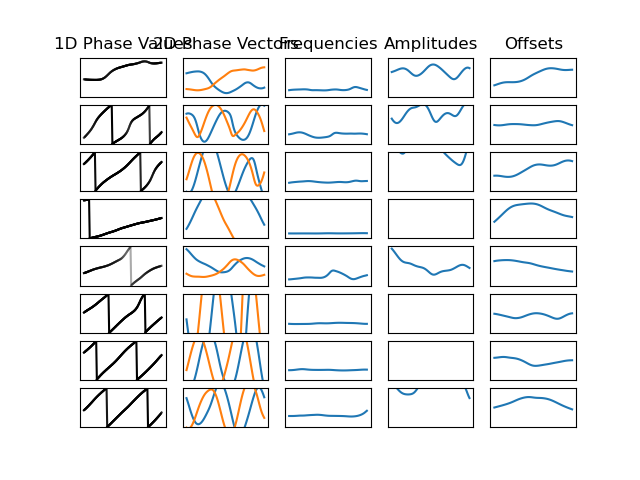
\includegraphics[width=\linewidth]{images/phase_bias_frequency_amplitudes_offsets.png}
	\caption{Các tham số đã học cho pha, biên độ, tần số và độ lệch cho một khoảng thời gian chuyển động cố định trong quá trình huấn luyện mạng để tái tạo chuyển động đầu vào, và từ đó có thể xây dựng đa tạp pha.}
	\label{fig:phase_bias_frequency_amplitudes_offsets}
\end{figure}

%$$
%\Gamma(x) = A sin (2 \pi (Fx - S)) + B
%$$

%Diffusion \cite{ho2020denoising} là mô hình được lấy cảm hứng từ mô hình khuếch tán các chất trong hóa học.

\subsection{Phase Manifold}
\label{sec:summary_diffusion}

%\begin{figure*}
%	\centering
%	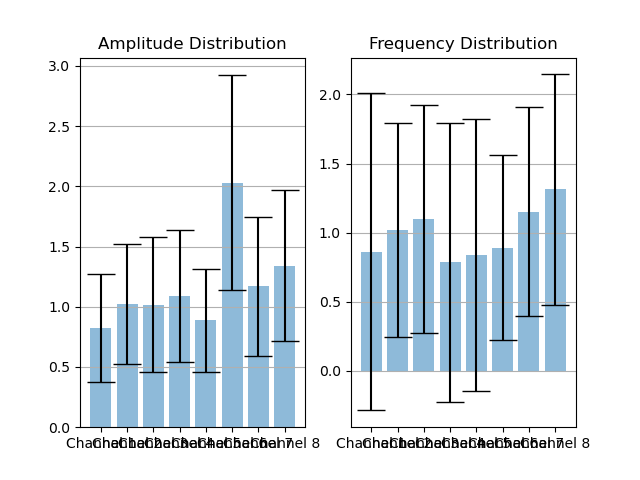
\includegraphics[width=0.8\linewidth]{images/distribution.png}
%	\caption{Phân phối của các biên độ và tần số của các kênh pha đã học. Mỗi kênh được điều chỉnh cho một khoảng biên độ và tần số cụ thể để phân tích chuyển động, hoạt động như một tập hợp các bộ lọc thông dải đã học. Lưu ý rằng không có các khoảng tham số được định nghĩa trước cho mỗi kênh pha, mà chúng được trích xuất theo nhu cầu của mô hình.}
%	\label{fig:distribution}
%\end{figure*}

\begin{figure}
	\centering
	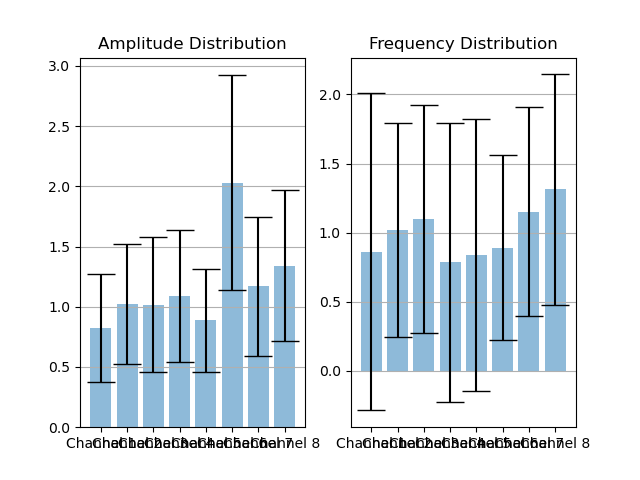
\includegraphics[height=10cm,width=\linewidth]{images/distribution.png}
	\caption{Phân phối của các biên độ và tần số của các kênh pha đã học. Mỗi kênh được điều chỉnh cho một khoảng biên độ và tần số cụ thể để phân tích chuyển động, hoạt động như một tập hợp các bộ lọc thông dải đã học. Lưu ý rằng không có các khoảng tham số được định nghĩa trước cho mỗi kênh pha, mà chúng được trích xuất theo nhu cầu của mô hình.}
	\label{fig:distribution}
\end{figure}

Chúng tôi sẽ mô tả cách mà đa tạp pha được hình thành bằng cách sử dụng các biến tiềm ẩn chu kỳ được tính toán với Mạng Tự Động Hóa Chu Kỳ. Sau khi huấn luyện mạng, các tham số chu kỳ cho một tập dữ liệu chuyển động không có cấu trúc có thể được tính toán cho mỗi khung hình bằng cách dịch Mạng Tự Động Hóa Chu Kỳ dọc theo các đường cong chuyển động. Các tham số chu kỳ đại diện cho tính chu kỳ cục bộ của các biến tiềm ẩn: sử dụng chúng, chúng tôi hình thành một đa tạp pha $\mathcal{P}$ có kích thước $\mathbb{R}^{2M}$, trong đó một mẫu tại khung hình $t$ được tính bằng

\begin{equation}
	\label{eq:phase_define}
	\mathcal{P}^{(t)}_{2i-1} = \textbf{A}^{(t)}_i \cdot \sin(2\pi \cdot \textbf{S}^{(t)}_i), \quad \mathcal{P}^{(t)}_{2i} = \textbf{A}^{(t)}_i \cdot \cos(2\pi \cdot \textbf{S}^{(t)}_i)
\end{equation}


\begin{figure}
	\centering
	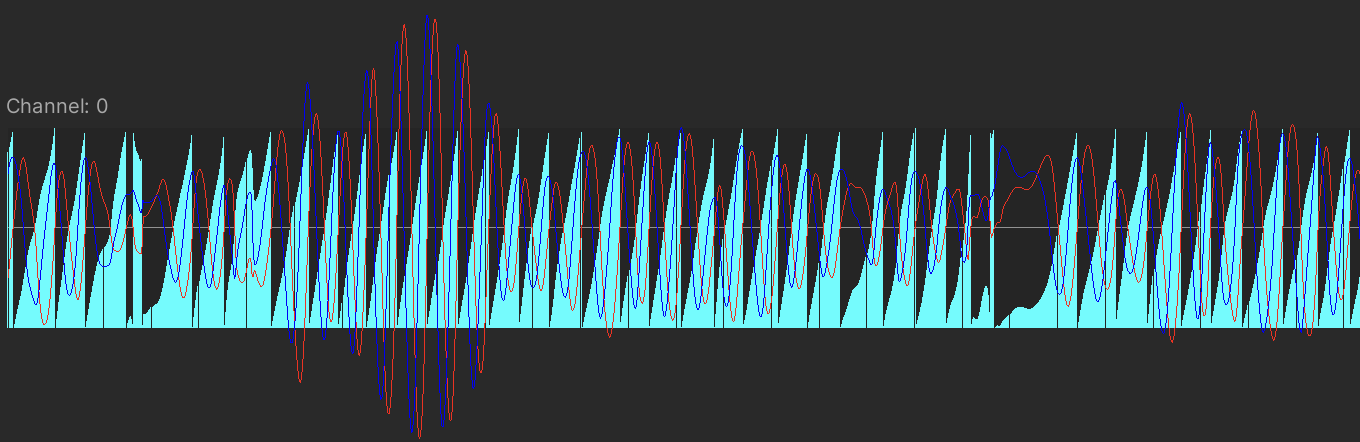
\includegraphics[width=\linewidth]{images/PhaseChannel.png}
	\caption{Phân phối của các biên độ và tần số của các kênh pha đã học. Mỗi kênh được điều chỉnh cho một khoảng biên độ và tần số cụ thể để phân tích chuyển động, hoạt động như một tập hợp các bộ lọc thông dải đã học. Lưu ý rằng không có các khoảng tham số được định nghĩa trước cho mỗi kênh pha, mà chúng được trích xuất theo nhu cầu của mô hình.}
	\label{fig:PhaseChannel}
\end{figure}


Các đặc trưng trong $\mathcal{P}$ mô tả tốt thời gian của khung hình trong chuyển động đầu vào $\textbf{X}$ và giúp rất nhiều trong việc căn chỉnh các chuyển động trong cùng một lớp hoặc giữa các lớp chuyển động khác nhau. Điều này có nghĩa là chúng có thể hoạt động hiệu quả như một đặc trưng đầu vào cho việc tổng hợp chuyển động thần kinh hoặc so khớp chuyển động, chúng tôi sẽ trình bày cách sử dụng và kết quả trong Mục 4 và Mục 5. Các biến pha của mười kênh trong một khoảng thời gian ngắn cho một đoạn clip chuyển động ví dụ được vẽ trong Hình 3. Có thể quan sát rằng mỗi kênh học các đặc trưng cho các tần số khác nhau, tương ứng với các tốc độ chuyển động khác nhau. Chúng tôi vẽ phân phối các biên độ và tần số của mỗi kênh trong Hình 4. Chúng tôi có thể quan sát rằng mỗi kênh pha học cách trích xuất các khoảng giá trị biên độ và tần số khác nhau trong các chuyển động. Hệ thống có thể mã hóa các chi tiết hoặc mẫu chuyển động khác nhau, điều này rất hữu ích cho việc căn chỉnh theo thời gian.

Khi có một chuỗi chuyển động, đặc trưng chu kỳ chuyển động mượt mà qua đa tạp pha. Vì biên độ và tần số của mỗi kênh pha có thể thay đổi theo thời gian, Mạng Tự Động Hóa Chu Kỳ có thể mã hóa các chuyển động không chu kỳ cũng như các chuyển động chu kỳ, chẳng hạn như chuyển tiếp từ một loại chuyển động này sang loại khác. Những chuyển tiếp không chu kỳ hoặc hành vi chuyển động như vậy có thể được quan sát dưới dạng biên độ tăng hoặc giảm cho các kênh khác nhau (ví dụ: một người đi bộ và bắt đầu vẫy tay), hoặc thay đổi không đồng bộ trong dịch pha hoặc tần số (ví dụ: chuyển tiếp giữa bước đi và bước chạy cho các loài bốn chân). Hình 5 minh họa những ví dụ như vậy nơi các pha có thể thể hiện các mẫu chu kỳ hoặc không chu kỳ trong suốt một đoạn clip chuyển động.



Lý do để định nghĩa đa tạp pha như trong phương trình (8) thay vì sử dụng riêng biệt tất cả các tham số như tần số, biên độ và pha là vì chúng tôi mong muốn các đặc trưng pha nhóm các hoạt ảnh theo cả không gian và thời gian. Các đặc trưng như tần số và biên độ vẫn gần như không thay đổi theo thời gian, và không giúp ích nhiều cho mục đích căn chỉnh. Biến đổi chúng thành một không gian hình cầu siêu thông qua phương trình (8) đạt được sự căn chỉnh không gian-thời gian như vậy, trong đó $A$ và $S$ định nghĩa điểm trong không gian đó và $F$ có thể được đại diện bởi một cửa sổ của các điểm như vậy. Phép biến đổi này cũng xây dựng một không gian nội suy liên tục: Trong khi các giá trị pha 1D là không liên tục và có thể trở nên không xác định nếu không có chuyển động nào được thực hiện, việc mã hóa chúng dưới dạng các vector 2D cho phép chuyển tiếp về gốc của đa tạp tại biên độ bằng không.

\subsection{Network Training}

Để huấn luyện Mạng Tự mã hóa Chu kỳ, chúng tôi sử dụng các quỹ đạo vận tốc khớp 3D làm đầu vào cho mạng, mỗi quỹ đạo được chuyển đổi vào không gian gốc của nhân vật [Holden et al. 2017]. Chúng tôi trừ đi giá trị trung bình dựa trên cửa sổ để căn giữa các đường cong chuyển động, nhưng không áp dụng bất kỳ phép tỷ lệ độ lệch chuẩn nào nhằm duy trì các khác biệt tương đối. Dữ liệu đầu vào bao gồm 60 khung hình (1 giây) mỗi khung ở quá khứ và tương lai xung quanh khung giữa với tần số 60 Hz. Điều này tạo ra một vector đầu vào $\textbf{X} \in \mathbb{R}^{3 \cdot J \times N}$, trong đó $J$ là số lượng khớp của nhân vật và $N$ (= 121) là số lượng mẫu thời gian.
Đối với bộ mã hóa $g$, chúng tôi sử dụng hai lớp tích chập, tạo ra một ánh xạ $(3 \cdot J \times N) \to (J \times N) \to (M \times N)$, để tính toán nhúng đường cong chuyển động. Mỗi lớp tích chập được theo sau bởi một phép chuẩn hóa theo lô (batch normalization) và hàm kích hoạt tanh. Vì chúng tôi thực hiện trực tiếp các phép toán trên không gian tiềm ẩn để trích xuất các tham số chu kỳ, chúng tôi nhận thấy rằng việc chuẩn hóa theo lô giúp ổn định quá trình huấn luyện cho nhiệm vụ này và giúp ngăn chặn sự phân phối không gian tiềm ẩn bị suy giảm hoặc mô hình bị quá khớp khi được huấn luyện quá lâu. Chúng tôi cũng áp dụng một phép chuẩn hóa theo lô cho vector dịch pha dự đoán trước khi tính toán góc có dấu của nó. Bộ giải mã $h$ lại bao gồm hai lớp tích chập để tính toán một ánh xạ $(M \times N) \to (J \times N) \to (3 \cdot J \times N)$, nhưng chỉ áp dụng phép chuẩn hóa theo lô và hàm kích hoạt tanh sau lớp giải chập đầu tiên và không áp dụng cho lớp đầu ra. Chúng tôi huấn luyện mạng của mình bằng bộ tối ưu AdamW [Loshchilov và Hutter 2019] trong 30 epoch, sử dụng tốc độ học và độ suy giảm trọng số đều là $10^{-4}$ và kích thước lô là 32. Việc huấn luyện trên GPU NVIDIA RTX 3090 thường mất chưa đầy một giờ cho các tác vụ nhỏ hơn.


\section{Motion Controllers}
\label{MotionControllers}

\subsection{Neural Motion Controller}

\begin{figure}
	\centering
	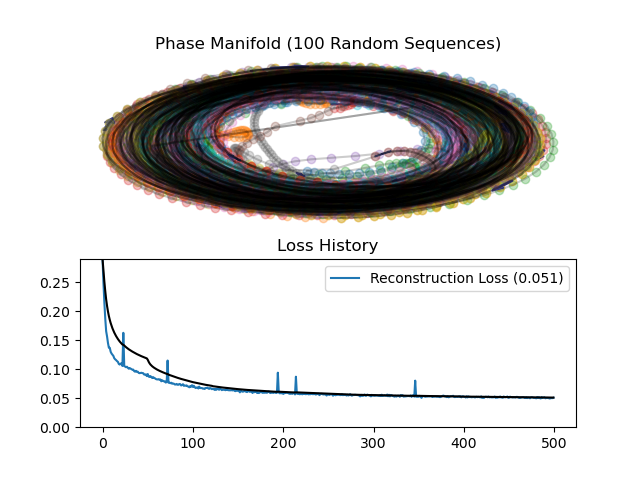
\includegraphics[]{images/PhaseManifold.png}
	\caption{Phân phối đặc trưng cho các miền chuyển động khác nhau trong không gian vận tốc (trên), không gian tiềm ẩn được học bởi mạng tích chập + mạng kết nối hoàn toàn (giữa) và không gian pha (dưới) được trực quan hóa bằng phép chiếu PCA 2D. Mỗi màu đại diện cho các tư thế từ một chuỗi chuyển động duy nhất mà được kết nối theo thời gian.}
	\label{fig:PhaseManifold}
\end{figure}


Đối với bộ điều khiển dựa trên mạng nơ-ron, chúng tôi phát triển một mô hình chuỗi thời gian dự đoán tư thế trong khung hình hiện tại dựa trên khung hình trước đó và các điều khiển của người dùng hiện tại. Mô hình được huấn luyện theo cách giám sát sử dụng dữ liệu ghi hình chuyển động. Chúng tôi sử dụng khung Mixture-of-Experts pha trộn trọng số tương tự như [Starke et al. 2020; Zhang et al. 2018], nhưng thay vì sử dụng các vận tốc hoặc pha địa phương dựa trên tiếp xúc làm đầu vào cho mạng gating, chúng tôi sử dụng các vectơ pha trên mặt phẳng pha (tức là, Eq. (8)) làm các đặc trưng đầu vào để tạo ra các chuyển động theo cách tự hồi quy. Việc cung cấp đặc trưng pha làm đầu vào giúp hệ thống căn chỉnh dữ liệu chuyển động theo dòng thời gian và cho phép nhân vật chuyển tiếp giữa các chuyển động một cách thực tế như chúng tôi đã trình bày trong Mục 5.

Hệ thống tự hồi quy cập nhật trạng thái pha của nhân vật cũng như chuyển động của nó. Hệ thống đầu tiên dự đoán các vectơ pha tiếp theo $P_{t+\Delta t}$, các biên độ $A_{t+\Delta t}$ và tần số $F_{t+\Delta t}$. Thay vì sử dụng trực tiếp các vectơ pha đã dự đoán, nó được cập nhật như sau:

\begin{equation}
	\label{eq:PhaseVector}
	\mathcal{P}_{t+\Delta t}^{\prime}=A_{t+\Delta t} \cdot I\left(R(\theta) \cdot \mathcal{P}_t, \mathcal{P}_{t+\Delta t}\right), \quad \theta=\Delta t \cdot 2 \pi \cdot F_{t+\Delta t}
\end{equation}

trong đó \(\Delta t\) là thời gian delta của khung hình, \(R\) là ma trận quay 2D, và \(I\) là nội suy tuyến tính hình cầu với trọng số 0.5 để cho phép pha trộn góc pha và độ lớn một cách riêng biệt. Việc cập nhật pha theo cách này buộc tần số tiến triển pha theo hướng mà mạng nơ-ron đã dự đoán. Tần số là một giá trị dương đồng nhất dễ dự đoán và giữ cho mạng di chuyển qua không gian pha theo một cách một chiều (xem Hình 6). Sơ đồ này ngăn chuyển động trở nên cứng nhắc hoặc bị kẹt theo thời gian, điều này là một vấn đề phổ biến được quan sát thấy đối với các bộ điều khiển nhân vật dựa trên dữ liệu.

Mạng gating chuyên gia học cách pha trộn 8 bộ trọng số chuyên gia và bao gồm hai lớp ẩn có kích thước 128. Mạng tạo chuyển động sử dụng hai lớp ẩn có kích thước 512. Tỉ lệ dropout được đặt thành 0.3, kích thước lô là 32, và cả tốc độ học và suy giảm trọng số đều được khởi tạo là \(10^{-4}\). Chúng tôi sử dụng bộ tối ưu AdamWR [Loshchilov và Hutter 2019] với lịch trình giảm nhiệt cosin và đặt số lần khởi động lại là 10, hệ số khởi động lại là 2.0, và huấn luyện mô hình trong 150 epoch. Việc huấn luyện mỗi mô hình yêu cầu từ 12 đến 48 giờ. Mạng được triển khai trong PyTorch và tạo ra một tệp ONNX có thể được chạy trong Unity để suy diễn bằng cách sử dụng thư viện Barracuda của nó.


\subsection{Motion Matching}

Trong bối cảnh của việc khớp chuyển động, các pha có thể được sử dụng theo cách tương tự như đối với các mạng nơ-ron và không yêu cầu thay đổi trong các quy trình công việc điển hình cho việc khớp chuyển động. Sự khác biệt chính là thay vì khớp các đặc trưng tư thế hoặc vận tốc có chiều cao hơn của trạng thái nhân vật hiện tại, hệ thống khớp các vectơ pha có chiều thấp hơn để tìm kiếm tư thế ở khung hình tiếp theo dựa trên các tín hiệu điều khiển của người dùng, chẳng hạn như quỹ đạo gốc. Chúng tôi trực quan hóa các đặc trưng pha và các đặc trưng vận tốc cho các chuyển động khác nhau trong Hình 6 (xem Mục 5.1 để biết thêm chi tiết). Khoảng cách Euclid giữa các điểm lân cận trong không gian pha liền kề với nhau là đồng nhất (hàng dưới cùng), điều này có nghĩa là các tư thế được khớp bởi việc khớp chuyển động sẽ có sự khác biệt tương tự về thời gian. Điều này cho phép

tổng hợp các chuyển tiếp chuyển động mượt mà và thực tế hơn với ít điều chỉnh tham số hơn, điều này không dễ dàng xảy ra khi khớp các đặc trưng tư thế Cartesian (hàng trên cùng) cần được chọn thủ công cho các khớp cụ thể (ví dụ: chân cho chuyển động) hoặc yêu cầu thêm bộ lọc.





%\subsection{Quá trình gây nhiễu (forward diffusion process)}
%
%Cho dữ liệu $x_{0}$ là được lấy từ dữ liệu thật $x_{0} \sim q(x)$, với mỗi bước ta sẽ thêm nhiễu vào đầu vào $x_{0}$ với tỷ lệ nhiều và ảnh gốc được kiểm soát bằng hệ số $\beta$:
%
%
%\begin{equation}
%	\label{eq:addgaussian}
%	\mathbf{x}_t = \sqrt{1 - \beta_t}\mathbf{x}_{t-1} + \sqrt{\beta_t} \boldsymbol{\epsilon}_{t-1}
%\end{equation}
%
%Trong đó, quá trình gây nhiễu từ $1 \to T$, với mỗi bước $t$ quá trình thêm nhiễu $\epsilon$ được điều khiển bằng $\beta_t$ theo phương sai $\{\beta_t \in (0, 1)\}_{t=1}^T$:
%
%\begin{equation}
%	\label{eq:forward_diffusion_process}
%	\begin{aligned}
%		q(\mathbf{x}_t \vert \mathbf{x}_{t-1}) &= \mathcal{N}(\mathbf{x}_t; \sqrt{1 - \beta_t} \mathbf{x}_{t-1}, \beta_t\mathbf{I}) \quad \\
%		q(\mathbf{x}_{1:T} \vert \mathbf{x}_0) &= \prod^T_{t=1} q(\mathbf{x}_t \vert \mathbf{x}_{t-1})
%	\end{aligned}
%\end{equation}
%
%Mục tiêu ở bước $t$ của hệ số $\sqrt{1 - \beta_t}$ và $\beta_t$ là để lần lượt giảm tỷ lệ của ảnh gốc $x_t$ và tăng dần nhiễu  $\boldsymbol{\epsilon}_{t-1}$, vì vậy $\beta_1 < \beta_2 < \dots < \beta_T$. Khi $T \to \infty$ thì $x_{T}$ sẽ hoàn toàn nhiễu (Isotropic Gaussian Distribution).
%
%
%Vì nhiễu $\boldsymbol{\epsilon}_{t-1}, \boldsymbol{\epsilon}_{t-2}, \dots \sim \mathcal{N}(\mathbf{0}, \mathbf{I})$ luôn luôn là phân phối chuẩn, và cho trước trong mọi bước $t$, nên ta có thể dễ dàng truy ngược được $x_t$ từ $x_0$. Bằng cách đặt $\alpha_t = 1 - \beta_t$ và $\bar{\alpha}_t = \prod_{i=1}^t \alpha_i$, từ công thức \ref{eq:addgaussian}, ta có hàm forward diffusion viết lại theo $\alpha$ như sau:
%
%\begin{equation}
%	\label{eq:tracexzero}
%	\begin{aligned}
%		\mathbf{x}_t 
%		&= \sqrt{\alpha_t}\mathbf{x}_{t-1} + \sqrt{1 - \alpha_t}\boldsymbol{\epsilon}_{t-1} \\
%		&= \sqrt{\alpha_t \alpha_{t-1}} \mathbf{x}_{t-2} + \sqrt{1 - \alpha_t \alpha_{t-1}} \bar{\boldsymbol{\epsilon}}_{t-2}
%		&= \sqrt{\bar{\alpha}_t}\mathbf{x}_0 + \sqrt{1 - \bar{\alpha}_t}\boldsymbol{\epsilon} \\
%		q(\mathbf{x}_t \vert \mathbf{x}_0) &= \mathcal{N}(\mathbf{x}_t; \sqrt{\bar{\alpha}_t} \mathbf{x}_0, (1 - \bar{\alpha}_t)\mathbf{I})
%	\end{aligned}
%\end{equation}
%
%
%\subsection{Quá trình khử nhiễu (denoising process)}
%\label{subsection:denoising_process}
%
%Quá trình khử nhiễu $p_\theta(\mathbf{x}_{t-1} \vert \mathbf{x}_t)$  ở bước thứ $t$ từ $T \to 1$ được bắt đầu từ $x_T$ là hoàn toàn nhiễu $\mathcal{N} (\mathbf{0}, \mathbf{I})$. Ta sẽ dùng một neural network $f_{\theta} (x_t, t)$ để dự đoán nhiễu $\hat{\epsilon} = f_{\theta}(x_t, t)$ đã được thêm vào để được $x_{t-1}$ từ $x_t$.
%. Quá trình khử nhiễu có trung bình $\boldsymbol{\mu}_\theta(\mathbf{x}_t, t) = {\frac{1}{\sqrt{\alpha_t}} \Big( \mathbf{x}_t - \frac{1 - \alpha_t}{\sqrt{1 - \bar{\alpha}_t}}  f_\theta(\mathbf{x}_t, t) \Big)}$ và độ lệch chuẩn $\boldsymbol{\Sigma}_\theta(\mathbf{x}_t, t)$ như sau:
%
%
%%\begin{equation} \mathrm{d}\mathbf{x} = [\mathbf{f}(\mathbf{x}, t) - g^2(t) \nabla_\mathbf{x} \log p_t(\mathbf{x})]\mathrm{d}t + g(t) \mathrm{d} \mathbf{w}.\label{rsde} \end{equation}
%
%% bằng cách lấy ảnh bị nhiễu trừ đi nhiễu dự đoán
%
%\begin{equation}
%	\label{eq:denoising_process}
%	\begin{aligned}
%		p_\theta(\mathbf{x}_{0:T})
%		&= p(\mathbf{x}_T) \prod^T_{t=1} p_\theta(\mathbf{x}_{t-1} \vert \mathbf{x}_t) \\
%		p_\theta(\mathbf{x}_{t-1} \vert \mathbf{x}_t) &= \mathcal{N}(\mathbf{x}_{t-1};  \boldsymbol{\mu}_\theta(\mathbf{x}_t, t), \boldsymbol{\Sigma}_\theta(\mathbf{x}_t, t))
%	\end{aligned}
%\end{equation}
%
%%Ta viết lại hàm denoising từ công thức \ref{eq:denoising_process}  theo $\alpha$ như sau:
%%$$
%%x_{t-1} = \frac{1}{\sqrt{\alpha_t}} \left( x_t - \frac{\sqrt{1 - \alpha_t}}{\sqrt{1 - \bar{\alpha}_t}} \epsilon_{\theta}(x_t, t) \right) + \sqrt{1 - \alpha_t} \tilde{\epsilon}_t
%%$$
%
%
%%\begin{equation}
%%	\label{eq:denoising_alpha}
%%	\begin{aligned}
%	%	p_\theta(\mathbf{x}_{t-1} \vert \mathbf{x}_t) &= \mathcal{N}(\mathbf{x}_{t-1}; \boldsymbol{\mu}_\theta(\mathbf{x}_t, t), \boldsymbol{\Sigma}_\theta(\mathbf{x}_t, t))
%	%\end{aligned} \\
%	% \bar{\boldsymbol{\mu}}_t (x_t, t) = \frac{1}{\sqrt{\alpha_t}} \Big( \mathbf{x}_t - \frac{1 - \alpha_t}{\sqrt{1 - \bar{\alpha}_t}} \boldsymbol{\epsilon}_t \Big)
%	%\end{equation}
%	
%	\subsection{Hàm mất mát $\mathcal{L}$ của mô hình diffusion}
%	
%	Như đã trình bày ở trên, mô hình diffusion sẽ học trọng số $\theta$ của hàm dự đoán lỗi $f_{\theta} (x_t, t)$. Trong quá trình denoising, ta sẽ tối ưu độ lỗi giữa nhiễu dự đoán $\boldsymbol{\epsilon}_\theta(\mathbf{x}_t, t)$ và nhiễu thực tế $\boldsymbol{\epsilon}_t$. Với mỗi bước thứ $t$ ta sẽ tối ưu hàm loss $\mathcal{L}_{t}$ để thu được trọng số $\theta$.
%	
%	\begin{equation}
%		\label{eq:diffusion_loss}
%		\begin{aligned}
%			\mathcal{L}_t
%			&= \mathbb{E}_{t \sim [1, T], \mathbf{x}_0, \boldsymbol{\epsilon}_t} \Big[\|\boldsymbol{\epsilon}_t - \boldsymbol{\epsilon}_\theta(\mathbf{x}_t, t)\|^2 \Big] \\
%			&= \mathbb{E}_{t \sim [1, T], \mathbf{x}_0, \boldsymbol{\epsilon}_t} \Big[\|\boldsymbol{\epsilon}_t - \boldsymbol{\epsilon}_\theta(\sqrt{\bar{\alpha}_t}\mathbf{x}_0 + \sqrt{1 - \bar{\alpha}_t}\boldsymbol{\epsilon}_t, t)\|^2 \Big]
%		\end{aligned}
%	\end{equation}
%	
%	Thay vì dùng neuron network để dự đoán phân bố của dữ liệu theo như hình \ref{fig:basic_diffusion}, mô hình diffusion sẽ dự đoán độ lỗi được thêm vào trong ảnh ở bước thứ $t$, với mỗi $t$ bước ta sẽ cần tối ưu hàm mất mát $\mathcal{L}_t$, hàm mất mát của mỗi bước sẽ tối ưu độ lỗi giữa nhiễu dự đoán $\hat{\epsilon_t}$ và nhiễu nhãn $\epsilon_t$ được thêm vào. Với $f_{\theta}(x_{t-1}, t)$ là một mô hình Unet dùng để mã hoá và giải mã dữ liệu để dự đoán nhiễu đã thêm vào dữ liệu.
%	
%	%Hàm loss
%	
%	
%	\subsection{Quá trình dự đoán trong mô hình diffusion}
%	
%	Sau khi thu được trọng số $\theta'$, ta sẽ dùng hàm denoising để khử nhiễu từ nhiễu $x_T \sim \mathcal{N} (\mathbf{0}, \mathbf{I})$.
%	Quá trình biến đổi từ nhiễu hoàn toàn $x_{T}$ sang dự đoán $\hat{x_0}$ như sau:
%	%với $t$ là một vector đã được nhúng vị trí bằng thuật toán nhúng
%	
%	\begin{equation}
%		\label{eq:adddenoising}
%		x_{t-1} = \frac{1}{\sqrt{\alpha_t}} \left( x_t - \frac{1- \alpha_t}{\sqrt{1 - \bar{\alpha}_t}} f_{\theta'}(x_t, t) \right) + \sqrt{1 - \alpha_t} \tilde{\epsilon}_t
%	\end{equation}
%	
%	Lưu ý rằng $\tilde{\epsilon}_t$ là nhiễu cố định $\epsilon_t$ giống với nhiễu trong quá trình forward diffusion \ref{subsection:denoising_process} ở công thức  \ref{eq:addgaussian}.
%
	
% GAT
%% \section*{Mô hình sinh cử chỉ OHGesture}

% \section*{3 Phương Pháp Của Chúng Tôi}
% Diffusion là mô hình đằng sau các thành công của  Stable Diffusion, Midjourney và DALL-E trong việc tạo ra các tấm ảnh siêu thực.


%. Biếm tiềm ẩm ở đây là cử chỉ và điều kiện là cảm xúc. 
%Kiến trúc của OHGesture được trình bày như hình \autoref{fig:diffusion_forward}.


\section{Mô hình của đề xuất OHGesture}
\label{sec:ohgesture}

\begin{figure}
	\centering
	\includegraphics[width=\linewidth]{images/diffusion_forward}
	\caption{Minh hoạ quá trình khử nhiễu (denoising) cử chỉ}
	\label{fig:diffusion_forward}
\end{figure}

Mô hình \textbf{OHGesture} của chúng tôi áp dụng mô hình khuếch tán \cite{ho2020denoising} với điều kiện \cite{ho2022classifier} (Classifier-Free Diffusion Guidance). Trong đó $x_0$ là chuỗi cử chỉ $g \in \mathbb{R}^{N \times 1141}$, với điều kiện $c$bao gồm  .
Với đầu vào bao gồm cử chỉ khởi tạo $x_{\text{seed}}$, âm thanh $a$ và văn bản $t$.
% với biến tiềm ẩn   (diffusion latent variable)
Mô hình diffusion bao gồm hai quá trình: quá trình tạo nhiễu (diffusion) $q$ và quá trình khử nhiễu (denoising process) $p_{\theta}$. 
Trước tiên chúng tôi trình bày trước về phương pháp nền tảng (baseline) của mô hình diffusion.

\subsection{Quá trình trích xuất đặc trưng}

Dữ liệu để học của chúng tôi được lấy từ tập dữ liệu BEAT (Body-Expression-Audio-Text)
\cite{liu2022beat}. Tương tự mô hình DiffuseStyleGesture \cite{yang2022DiffuseStyleGestureplus} chúng tôi cũng sử dụng đầu vào bao gồm âm thanh, cử chỉ và cảm xúc, ngoài ra chúng tôi sử dụng thêm dữ liệu văn bản.

\begin{itemize}
	\item \textbf{Cử chỉ}: Cử chỉ ground truth là dữ liệu bao gồm 75 khớp xương được trình bày ở công thức \ref{eq:gesturevector}. Chúng tôi cắt $N_{\text{seed}} = 8$ frame đầu để làm cử chỉ khởi tạo và $N$ frame tiếp theo làm cử chỉ để dự đoán theo âm thanh và văn bản.
	
%	\item\textbf{Âm thanh}: Âm thanh sẽ được dùng làm đặc trưng để sinh cử chỉ, Chúng tôi sử dụng các mô hình Pretrain có sẵn như WavLM \cite{chen2022wavlm} để trích xuất đặc trưng âm thanh. 
%	Chúng tôi kết hợp thêm các đặc trưng về MFCC, Mel-Spectrum, Pitch, Enery và Onsets \cite{bello2005tutorial}
  \item \textbf{Âm thanh}: Tất cả dữ liệu âm thanh được giảm số sample rate (downsampled) xuống $16 \mathrm{kHz}$ và các vector tiềm ẩn được lấy từ các mô hình pre-train của WavLM Large \cite{chen2022wavlm}. Chúng tôi sử dụng nội suy tuyến tính (interpolation) để căn chỉnh đặc trưng của vector tiềm ẩn trong WavLM và cử chỉ $x_{0}$ theo chiều thời gian thành $20fps$, sau đó sử dụng một lớp tuyến tính để giảm kích thước của đặc trưng xuống còn 64 tạo thành chuỗi đặc trưng âm thanh cuối cùng $\mathbf{A}$.
		
	\item \textbf{Cảm xúc}: Cảm xúc bao gồm 6 cảm xúc khác nhau được biểu diễn thành một vector theo phương pháp one-hot encoding.
	
	\item \textbf{Văn bản}: Văn bản được trích xuất thông qua mô hình FastText \cite{yoon2022genea} để lấy được vector word embedding.
	
	\item \textbf{Cử chỉ nhiễu} (Noisy gesture): khi huấn luyện, $x_{t}$ là cử chỉ nhiễu có cùng kích thước như cử chỉ gốc $x_{0}$ sẽ được sinh ngẫu nhiên từ phân phối chuẩn $\mathcal{N}(0, \mathbf{I})$. Khi sinh ngẫu nhiên, cử chỉ nhiễu ban đầu $x_{T}$ được lấy mẫu từ phân phối chuẩn tiêu chuẩn và các $x_{t}, t<T$ khác là kết quả của bước làm nhiễu trước đó. Sau đó, kích thước được điều chỉnh thành 256 như $\mathbf{G}$ bằng lớp linear.
	
\end{itemize}

%\item Bước làm nhiễu: Trong quá trình huấn luyện, bước làm nhiễu $t$ được lấy mẫu từ phân phối chuẩn của $\{1,2, \ldots, T\}$, với mã hóa vị trí (position encoding) giống như mô hình Transformer \cite{vaswani2017attention}, sau đó được ánh xạ vào không gian $\mathbf{T}$ có kích thước 256 bằng một mạng perceptron nhiều lớp (MLP).
%
%
%
%\item Cảm xúc: Các cảm xúc của cử chỉ được biểu diễn dưới dạng vectơ one-hot encoding, tức thành vector toàn bộ là số $0$ và vị trí có cảm xúc tương ứng có vị trí là $1$, vector one-hot encoding được ánh xạ vào không gian có kích thước 64 $\mathbf{S}$ thông qua một lớp tuyến tính.
%
%\item Cử chỉ khởi tạo: Cử chỉ khởi tạo giúp tạo ra sự chuyển tiếp mượt mà giữa các lần sinh liên tiếp \cite{yoon2020speech}. Cử chỉ khởi được cắt ngắn xuống $g \in$ $\mathbb{R}^{(8+N) \times 1141}$. Trong quá trình training, $8$ frame đầu tiên của cử chỉ $g$ được sử dụng làm cử chỉ khởi tạo $d$ và $N$ frame còn lại được sử dụng làm cử chỉ thật $x_{0}$ để tính hàm loss $\mathcal{L}$. Sau đó, chúng tôi ánh xạ các đặc trưng của cử chỉ khởi tạo $d$ vào không gian $\mathbf{D}$ có kích thước $192$ chiều bằng một lớp tuyến tính. 
%Kết quả cử chỉ được sinh ra trong $4$ giây, và vì cử chỉ sinh ra được chạy ở $20 \mathrm{fps}$ (tương đương 20 khung hình mỗi giây) nên kích thước $N=80$.

%\section{Mô hình diffusion cho bài toán sinh cử chỉ}

\begin{figure}
	\centering
	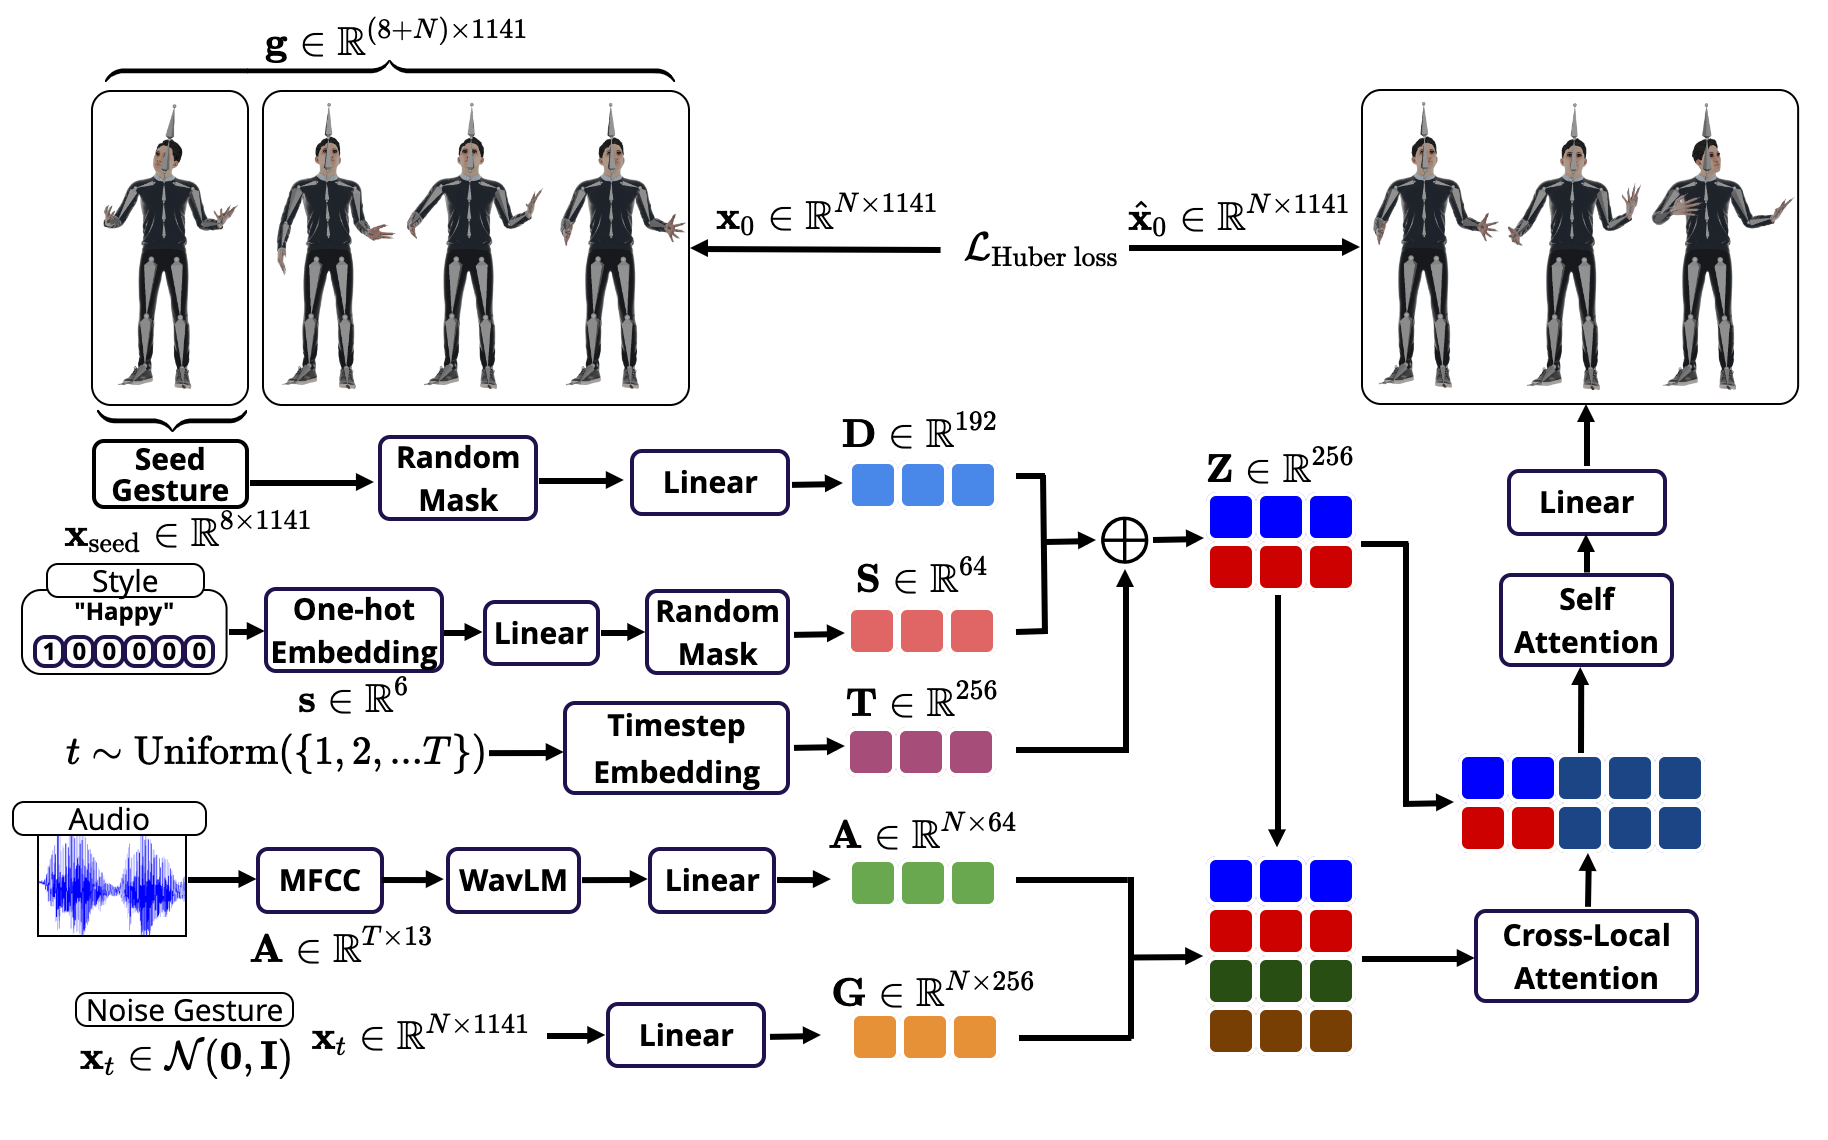
\includegraphics[width=\linewidth]{images/architecture_diffusion}
	\caption{Kiến trúc OHGesture}
	\label{fig:architecturediffusion}
\end{figure}


% Ý tưởng của chúng tôi là tạo ra các cử chỉ bằng một mô hình diffusion \cite{ho2020denoising} bằng cách học cách dần dần Denoise từ nhiễu hoàn toàn. Như được thể hiện trong Hình 2, mô hình diffusion bao gồm hai phần: quá trình tiến lùi (quá trình diffusion)  và quá trình ngược lại (quá trình Denoise).

%\subsection{Quá Trình Gây Nhiễu (Diffusion)}
%
%Quá trình diffusion $q$ được mô hình hóa như là một quá trình Markov với đầu vào lần lượt được thêm nhiễu, và sau đó mô hình lần lượt từng bước học để có thể tái tạo lại cử chỉ ban đầu.
%Trong bài toán sinh cử chỉ, đầu vào là các điểm trên tọa độ 3D, gọi là keypoint $x$, với $x_{0} \sim q\left(x_{0}\right)$ và $q\left(x_{0}\right)$ là phân phối của dữ liệu thực tế.
%Trong đó mỗi bước phương sai được thay đổi theo hệ số $\beta_{1}, \beta_{2}, \ldots, \beta_{T}$ $\left(0<\beta_{1}<\beta_{2}<\cdots<\beta_{T}<1, T\right)$, chúng tôi thêm nhiễu Gaussian
%
%\begin{equation} \label{eq:gaussian}
%q\left(x_{t} \mid x_{t-1}\right)=\mathcal{N}\left(x_{t} ; \sqrt{1-\beta_{t}} x_{t-1}, \beta_{t} \mathbf{I}\right)
%\end{equation}
%
%vào cử chỉ tại mỗi thời điểm $t$ lần lượt, và sau khi nhiễu Guassian được thêm vào đến bước $T$ đủ lớn, đến khi kết quả trở nên nhiễu hoàn toàn và không thể phân biệt được với kết quả ban đầu.

%\subsection{Quá Trình Khử Nhiễu (Denoise)}
%
%Quá trình Denoise $p_{\theta}$ là quá trình học tham số $\theta$ thông qua một mạng neural. Giả sử quá trình Denoise cũng tuân theo phân phối Gaussian, tức là nhiễu $x_{t}$ tại thời điểm $t$ được sử dụng để học $\mu_{\theta}, \Sigma_{\theta}$, sau đó
%
%\begin{equation} \label{eq:diffusion}
%p_{\theta}\left(x_{t-1} \mid x_{t}\right)=\mathcal{N}\left(x_{t-1} ; \mu_{\theta}\left(x_{t}, t\right), \Sigma_{\theta}\left(x_{t}, t\right)\right)
%\end{equation}
%
%Để thuận tiện cho việc tính toán, ta cho $\alpha_{t}=1-\beta_{t}$ và viết gọn lại $\bar{\alpha}_{t}=\prod_{i=1}^{T} \alpha_{i}$. Sau đó, cử chỉ nhiễu $x_{t}$ tại thời điểm $t$ có thể được viết lại như sau:
%
%\begin{equation} \label{eq:denoisevariance}
%q\left(x_{t} \mid x_{0}\right)=\mathcal{N}\left(x_{t} ; \sqrt{\bar{\alpha}_{t}} x_{0},\left(1-\bar{\alpha}_{t}\right) \mathbf{I}\right)
%\end{equation}
%
%Mô hình học bằng cách tối ưu hóa bằng cách giảm thiểu sự khác biệt giữa nhiễu thực sự $\epsilon$ và nhiễu được dự đoán $\epsilon_{\theta}\left(x_{t}, t\right)$ \cite{ho2020denoising}. Khi lấy mẫu, chúng ta có thể học giá trị trung bình $\mu_{\theta}\left(x_{t}, t\right)=\frac{1}{\sqrt{\alpha_{t}}}\left(x_{t}-\frac{\beta_{t}}{\sqrt{1-\bar{\alpha}_{t}}} \epsilon_{\theta}\left(x_{t}, t\right)\right)$ với phương sai cố định.

\subsection{Sinh cử chỉ với điều kiện}

Mục tiêu của chúng tôi là tổng hợp một cử chỉ con người $x^{1: N}$ có độ dài $N$ dựa trên điều kiện $c$. Trong mô hình OHGesture, tương tự như các phương pháp \cite{ramesh2022hierarchical} \cite{tevet2022human}, chúng tôi dự đoán dự liệu thật thay vì dự đoán nhiễu $\epsilon_{\theta}\left(x_{t}, t\right)$ như \cite{ho2020denoising}. Quá trình khử nhiễu (Denoise) tái tạo dữ liệu gốc $x_{0}$ dựa trên nhiễu đầu vào $x_{t}$, bước làm nhiễu $t$ và điều kiện $c$

\begin{equation} \label{eq:condition}
\hat{x}_{0}=\text { Denoise }\left(x_{t}, t, c\right)
\end{equation}

Sau đó, hàm khử nhiễu có thể được huấn luyện bằng cách tối ưu hóa hàm Huber loss \cite{huber1992robust} giữa các cử chỉ dự đoán $\hat{x}_{0}$ và các cử chỉ thực tế $x_{0}$ trên các tập huấn luyện:

\begin{equation} \label{eq:huberloss}
\mathcal{L}=E_{x_{0} \sim q\left(x_{0} \mid c\right), t \sim[1, T]}\left[\operatorname{HuberLoss}\left(x_{0}-\hat{x}_{0}\right)\right]
\end{equation}

\section{Áp dụng cơ chế Attention cho bài toán sinh cử chỉ}

\subsection{Hàm xử lý đặc trưng của quá trình khử nhiễu}

Như kiến trúc \textbf{OHGesture} trình bày trong hình \autoref{fig:architecturediffusion}, cử chỉ được tạo ra dựa trên bước làm nhiễu $t$, cử chỉ nhiễu $x_{t}$ và điều kiện $c$ (bao gồm âm thanh $a$, cảm xúc $s$ và cử chỉ khởi tạo $d$ ). Đối với mỗi đặc trưng, quá trình sinh cử chỉ được xử lý như sau:


\subsection{Cơ chế Attention trong hàm khử nhiễu}

Chúng tôi thực hiện việc khử nhiễu với kiến trúc dựa trên cơ chế attention. Để tính được tương quan của các đặc trưng xa, chúng tôi sẽ học để biểu diễn được các ngữ cảnh cực bộ (local context) theo \cite{rae2020transformers}.

Đầu tiên cử chỉ khởi tạo $\mathbf{D}$ và vector cảm xúc $\mathbf{S}$ được ghép lại với nhau để tạo thành một vectơ có kích thước 256, sau đó thêm vector làm nhiễu $\mathbf{T}$ để tạo thành vector $\mathbf{Z}$. 
Sau đó, vectơ $\mathbf{Z}$ và các bản sao của nó được ghép thành một chuỗi vector đặc trưng để khớp với dòng thời gian của âm thanh và đặc trưng cử chỉ, sau đó ghép với âm thanh $\mathbf{A}$ và cử chỉ $\mathbf{G}$ để làm đầu vào cho lớp local attention (chú ý cục bộ). 
Phương pháp sinh cử chỉ song hành với âm thanh của chúng tôi sử dụng lớp Local Attention được lấy ý tưởng từ phương pháp Routing Transformer \cite{roy2021efficient}, mà cho thấy rằng local attention quan trọng trong việc xây dựng biểu diễn trung gian, như được thể hiện trong Hình 3(c).

Sau đó, chúng tôi nối đầu ra của lớp local attention với $\mathbf{Z}$ và đưa vào lớp self-attention, như được thể hiện trong \autoref{fig:architecturediffusion}. Cơ chế self-attention tương tự như trình mã hóa (encoding) của Transformer \cite{vaswani2017attention}, giúp tính toán được mối liên hệ giữa các chuỗi dữ liệu với công tức sau:


\begin{equation} \label{eq:attention}
\operatorname{Attention}(\mathbf{Q}, \mathbf{K}, \mathbf{V}, \mathbf{M})=\operatorname{softmax}\left(\frac{\mathbf{Q} \mathbf{K}^{T}+\mathbf{M}}{\sqrt{C}}\right) \mathbf{V}
\end{equation}

trong đó $\mathbf{Q}, \mathbf{K}, \mathbf{V}$ là vector query, key và value từ dữ liệu đầu vào và $\mathbf{M}$ là mặt nạ (mask) giúp xác định loại của cơ chế attention, bao gồm \textit{full self-attention}, \textit{sliding window attention} và \textit{cross-local attention}. Để yếu tố thời gian không ảnh hưởng nhiều đến kết quả sinh cử chỉ, chúng tôi sử dụng cơ chế mã hóa vị trí tương đối (Relative Position Encoding - RPE) được trình bày trong phương pháp Reformer \cite{kitaev2020reformer}. Cuối cùng, đầu ra của self-attention được ánh xạ lại cùng kích thước như $x_{0}$ sau một lớp biến đổi tuyến tính.

\begin{figure*}[ht]
\begin{minipage}[b]{0.25\textwidth}
\centering
    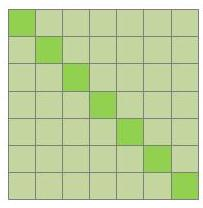
\includegraphics[width=\textwidth]{images/attention_full.jpg}
    \caption*{(a) full self-attention}
\end{minipage}
\hfill
\begin{minipage}[b]{0.25\textwidth}
\centering
    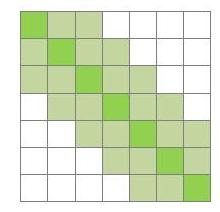
\includegraphics[width=\textwidth]{images/attention_sidewindow.jpg}
    \caption*{(b) sliding window attention}
\end{minipage}
\hfill
\begin{minipage}[b]{0.25\textwidth}
\centering
    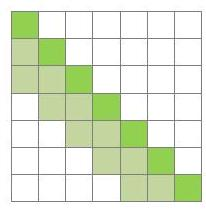
\includegraphics[width=\textwidth]{images/cross_attention.jpg}
    \caption*{(c) cross-local attention}
\end{minipage}
% \label{fig:type_attention}
\caption[Các loại attention khác nhau (full self-attention, sliding window attention, cross-local attention)]{Các loại attention khác nhau được sử dụng trong các thí nghiệm của chúng tôi, trong đó (a) và (c) là cơ chế attention được sử dụng trong mô hình của chúng tôi và (b) là một mẫu được sử dụng để đánh giá trong thực nghiệm. Mỗi dòng tương ứng với input và mỗi cột tương ứng với output của mô hình}
\end{figure*}

% Phần 4.3. Các hàng đại diện cho các đầu ra và các cột đại diện cho đầu vào. Các hình vuông màu sáng tô màu cho các phần tử liên quan đến mỗi dòng đầu ra.


Các cơ chế attention khác nhau có thể được tạo ra bằng cách điều chỉnh lớp mask tương ứng $\mathbf{M}$, 
tương tự như phương pháp Longformer \cite{beltagy2020longformer} chúng tôi cũng thử nghiệm cơ chế \textit{sliding window attention}.

\subsection{Phương pháp sample cử chỉ}

Để có thể sinh cử chỉ với chiều dài tùy ý, chúng tôi cắt chuỗi ban đầu thành các đoạn ngắn có chiều dài $N$. Trong quá trình huấn luyện, cử chỉ khởi tạo đầu tiên có thể được tạo ra bằng cách lấy ngẫu nhiên cử chỉ từ tập dữ liệu hoặc từ lấy trung bình từ đoạn cắt được. Cụ thể ở đây, sẽ lấy góc quay trung bình trong các đoạn đã cắt được. Tiếp theo chúng ta chỉ việc lấy lần lượt các frame đã sinh ra và chọn $8$ frame cuối cùng làm cử chỉ khởi tạo ở lượt tiếp theo. Đối với mỗi đoạn đã cắt ra, cử chỉ $x_{t}$ lần lượt sẽ được áp dụng hàm khử nhiều $\hat{x}_{0} = Denoise \left(x_{t}, t, c\right)$ cho đến khi được  $x_{t-1}$, và $x_{t-1}$ sẽ tiếp tục được làm khử nhiễu cho đến bước khử nhiễu $t=T$ sẽ đạt được $x_{0}$ như kiến trúc trong phần \autoref{fig:architecturediffusion}.


% chúng tôi , trong mỗi bước làm nhiễu $t$, chúng tôi dự đoán cử chỉ sạch  $=$  $\left(x_{t}, t, c\right)$, và thêm nhiễu vào bước làm nhiễu $x_{t-1}$ sử dụng Phương trình (1) với quá trình trải đều. Quá trình này được lặp lại từ $t=T$ cho đến khi đạt được $x_{0}$ (Hình 2 dưới cùng).

\section{Điều khiển cảm xúc trong bài toán sinh cử chỉ}

\begin{figure}[htbp]
    \centering
    \begin{subfigure}[b]{0.3\textwidth}
         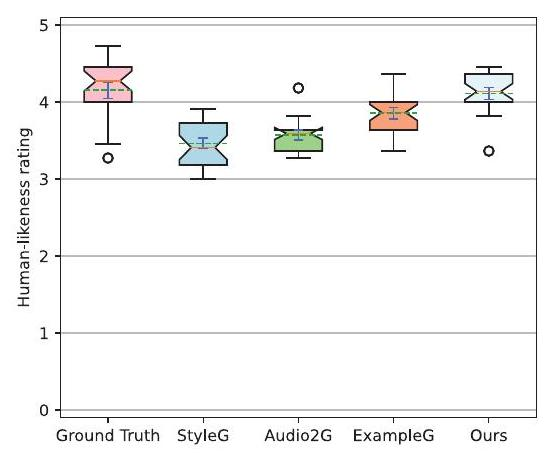
\includegraphics[width=\textwidth]{images/humanlike_score.jpg}
        \caption*{(a) Biểu đồ hộp của đánh giá về tính giống với con người}
    \end{subfigure}
    \hfill
    \begin{subfigure}[b]{0.3\textwidth}
        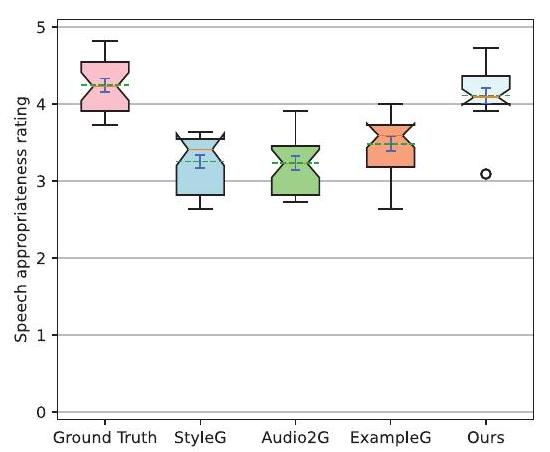
\includegraphics[width=\textwidth]{images/speech_score.jpg}
         \caption*{(b) Biểu đồ hộp của đánh giá về tính phù hợp giữa cử chỉ và âm thanh.}
    \end{subfigure}
    \hfill
    \begin{subfigure}[b]{0.3\textwidth}
        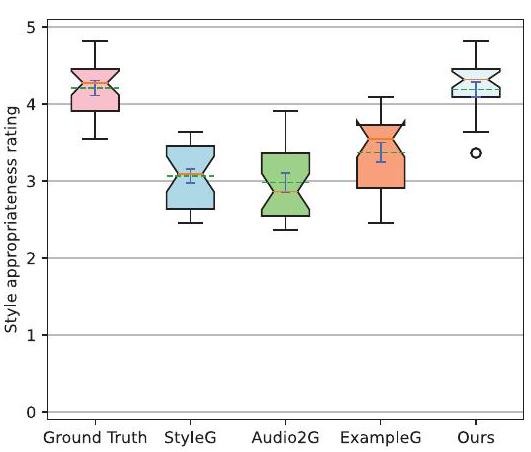
\includegraphics[width=\textwidth]{images/style_score.jpg}
        \caption*{(c) Biểu đồ hộp của đánh giá về tính phù hợp giữa cử chỉ và cảm xúc}
    \end{subfigure}
    \caption[Biểu đồ hộp mô tả kết quả so sánh MOS]{Biểu đồ hộp mô tả kết quả so sánh MOS cho các mô hình khác nhau trong các chiều khác nhau. Hộp mở rộng từ phân vị thứ nhất thấp nhất (Q1) đến phân vị thứ ba lớn nhất (Q3) của dữ liệu. Đường đỏ chỉ là giữa. Các khe nhỏ biểu thị khoảng tin cậy $95\%$ (CI) xung quanh giữa. Khi CI nhỏ hơn Q1 hoặc lớn hơn Q3, khe mở rộng ra khỏi hộp, tạo ra một hình dáng "lật" độc đáo. Chúng tôi cũng đã đánh dấu giá trị trung bình và khoảng tin cậy $95\%$ của nó trong hình với đường nét đứt màu xanh lá cây và đường dọc màu xanh lam, tương ứng.}
    \label{fig:3col}
\end{figure}


Ở các bước trên mô hình đã có thể học được cách sinh cử chỉ, nhưng để mô hình có thể học được các cảm xúc ở các tình huống khác nhau sẽ được giải quyết bằng cách tham số hóa và lần lượt thay đổi từng cảm xúc để sao cho khi thay đổi cảm xúc thì kết quả dự đoán phải có cảm xúc tương ứng.
Tham số để điều khiển ở đây là $c$, việc điều khiển ở đây không chỉ có thể là âm thanh $a$ mà còn là cảm xúc $s$ hoặc cử chỉ khởi tạo $d$, v.v. Chúng tôi tham khảo phương pháp của \cite{ho2022classifier}, \cite{tevet2022human}, bằng cách thêm một lớp mặt nạ ngẫu nhiên (random mask) trên các vector đặc trưng của cử chỉ khởi tạo $d$ và cảm xúc $s$ vào mô hình như hình minh họa \autoref{fig:architecturediffusion} để giúp kiểm soát chính xác việc mô hình có thể học được các đặc trưng ở các điều kiện khác nhau. Khi đó, mô hình chỉ việc thay đổi nhãn tương ứng với lớp mask đã lấy ngẫu nhiên để mô hình có thể tối ưu theo các điều kiện khác nhau. Khi đó hàm khử nhiễu $\text{Denoise} \left(x_{t}, t, c_{1}\right), c_{1}=[d, s, a]$ và hàm khử nhiễu mà không có điều kiện $\text{Denoise} \left(x_{t}, t, c_{2}\right), c_{2}=[\varnothing, \varnothing, a]$ sẽ được tối ưu trong quá trình huấn luyện, theo công thức

\begin{equation} \label{eq:denoise}
\hat{x}_{0 \gamma, c_{1}, c_{2}}=\gamma \text{Denoise} \left(x_{t}, t, c_{1}\right)+(1-\gamma) \text{Denoise} \left(x_{t}, t, c_{2}\right)
\end{equation}


Trong thực tế, hàm Denoise học cả phân phối có điều kiện và không có điều kiện bằng cách ngẫu nhiên phần mask $10 \%$ của các mẫu bằng các mask theo phân phối Bernoulli. Sau đó, đối với kiểu $s$ trong điều kiện, chúng ta có thể tạo ra cử chỉ được kiểm soát kiểu khi lấy mẫu bằng cách nội suy hoặc thậm chí là dự đoán hai biến thể bằng cách sử dụng $\gamma$, như $c_{1}=\left[d, s_{1}, a\right], c_{2}=\left[d, s_{2}, a\right]$

% \begin{figure*}[ht]
% \begin{minipage}[b]{0.3\textwidth}
% \centering
%     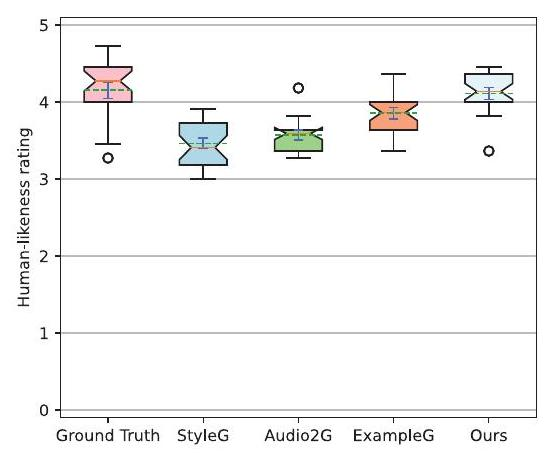
\includegraphics[width=\textwidth]{images/humanlike_score.jpg}
%     \caption*{(a) Biểu đồ hộp của đánh giá về tính giống với con người}
% \end{minipage}
% \hfill
% \begin{minipage}[b]{0.3\textwidth}
% \centering
%     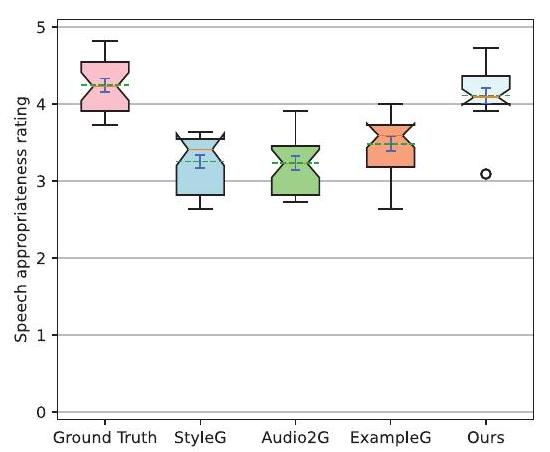
\includegraphics[width=\textwidth]{images/speech_score.jpg}
%     \caption*{(b) Biểu đồ hộp của đánh giá về tính phù hợp giữa cử chỉ và âm thanh.}
% \end{minipage}
% \hfill
% \begin{minipage}[b]{0.3\textwidth}
% \centering
%     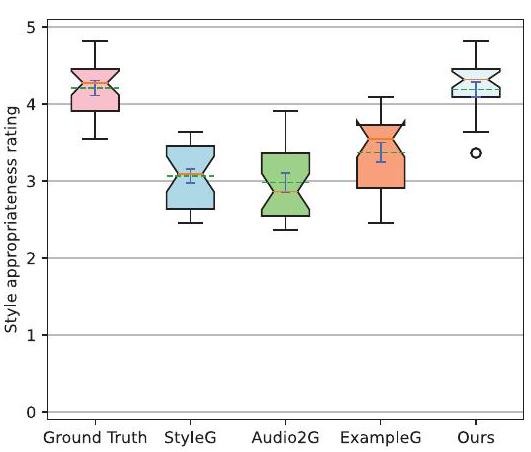
\includegraphics[width=\textwidth]{images/style_score.jpg}
%     \caption*{(c) Biểu đồ hộp của đánh giá về tính phù hợp giữa cử chỉ và cảm xúc}
% \end{minipage}
% \label{fig:gesture_score}
% \caption{Biểu đồ hộp mô tả kết quả so sánh MOS cho các mô hình khác nhau trong các chiều khác nhau. Hộp mở rộng từ phân vị thứ nhất thấp nhất (Q1) đến phân vị thứ ba lớn nhất (Q3) của dữ liệu. Đường đỏ chỉ là giữa. Các khe nhỏ biểu thị khoảng tin cậy $95\%$ (CI) xung quanh giữa. Khi CI nhỏ hơn Q1 hoặc lớn hơn Q3, khe mở rộng ra khỏi hộp, tạo ra một hình dáng "lật" độc đáo. Chúng tôi cũng đã đánh dấu giá trị trung bình và khoảng tin cậy $95\%$ của nó trong hình với đường nét đứt màu xanh lá cây và đường dọc màu xanh lam, tương ứng.}
% \end{figure*}


% Hình 4: Biểu đồ hộp thể hiện kết quả so sánh của MOS cho các mô hình khác nhau trong các chiều không gian khác nhau. Hộp mở rộng từ phần tư dưới thứ nhất (Q1) đến phần tư lớn thứ ba (Q3) của dữ liệu. Đường đỏ chỉ ra trung vị. Các rãnh biểu thị khoảng tin cậy $95 \%$ (CI) xung quanh trung vị. Khi CI ít hơn Q1 hoặc lớn hơn Q3, rãnh mở rộng ra ngoài hộp, tạo cho nó một diện mạo "lật" độc đáo. Chúng tôi cũng đã đánh dấu giá trị trung bình và CI $95\%$ của nó trong hình với một đường kẻ xanh lá cây đứt và một đường kẻ đứt màu xanh dương, tương ứng.

% \begin{equation}
% \left[\mathbf{r}_p, \mathbf{r}_r, \dot{\mathbf{r}}_p, \dot{\mathbf{r}}_r, \rho_p, \rho_r, \dot{\rho}_p, \dot{\rho}_r, g_d\right]
% \end{equation}


% Mô hình OHGesture được dựa trên mô hình QPGesture \cite{yang2023qpgesture} với nền tảng chính của phương pháp dựa trên mô hình VQ-VAE là mã hóa (encode) và giải mã (decode) dữ liệu hay nói cách khác chúng ta sẽ biểu diễn toàn bộ dữ liệu ở chiều dữ liệu thấp hơn và sau đó biểu diễn ngược trở lại kích thước ban đầu. Dữ liệu được biểu diễn thành các vùng trong không gian, với mỗi vùng có một đại diện tương ứng. Từ các địa diện ta có thể mã hóa ngược trở lại để chọn ra các ứng viên cử chỉ theo ngữ nghĩa (dữ liệu văn bản) hoặc nhịp điệu lời nói (dữ liệu âm thanh).
% Dựa trên hai cử chỉ ứng viên (gesture candidate), ta trích xuất ra pha dựa trên vận tốc xoay của các các khớp khi di chuyển và dựa trên pha hiện tại của cử chỉ khởi tạo, ta sẽ chọn được cử chỉ có pha gần nhât hay phù hợp nhất để chọn ra chuỗi cử chỉ cuối cùng.

% Cụ thể quá trình huấn luyện của mô hình bao gồm các quá trình như sau: Lượng tử hóa (Quantization), Ghép các chuyển động cử chỉ (Motion Matching), Điều hướng dựa theo pha của cử chỉ (Phrase Guided).

% Kiến trúc mô hình được trình bày minh họa trong hình \autoref{fig:architecturediffusion}.








% \subsection{Lượng tử hóa (Quantization)}
% % Learning a discrete latent space representation

% Lượng tử hóa là việc học để biểu diễn dữ liệu trong không gian rời rạc (discrete latent space representation). Ta sẽ biểu diễn dữ liệu lên không gian tiềm ần (latent space).
% Mục tiêu của việc lượng tử hóa là biểu diễn dữ liệu dưới số chiều thấp hơn hay chấm điểm/đánh giá dựa trên các đặc trưng của dữ liệu, từ đó dùng các điểm đã đánh giá để so sánh với nhau. Sau khi so sánh đánh giá, ta chọn được một ứng viên tốt nhất, từ ứng viên tốt nhất ta sẽ học để giải mã (decode) ngược trở lại dữ liệu ban đầu.

% Dữ liệu đầu vào được lượng tử hóa bao gồm âm thanh, cử chỉ và văn bản. Trong bài toán sinh cử chỉ, chúng tôi chỉ tập trung vào việc xử lý dữ liệu dựa trên cử chỉ nên đôi với dữ liệu văn bản và âm thanh, ta chỉ sử dụng lại các mô hình pre-train có sẵn. Với âm thanh chúng tôi sử dụng mô hình VQ-Wave2Vec \cite{baevski2019vq} để biểu diễn các dữ liệu âm thanh thành các latent vector. Hàm lượng tử hóa âm thanh là hàm $f_{quant\_audio} : \mathbf{A} \mapsto \mathbf{Z_{audio}}$ trong đó $\textbf{A}$ là các chuỗi các âm thanh sẽ được mã hóa lên vector lantent $\textbf{Z}$. Với $\textbf{Z_{audio}} \in \mathcal{Z}_a$.

% Đối với văn bản, chúng tôi sử dụng mô hình Sentene BERT \cite{reimers2019sentence} để biểu diễn các dữ liệu văn bản thành các vector tiềm ẩn. Hàm để nhúng các dữ liệu văn bản thành các vector là hàm $f_{embedding\_text} : \mathbf{T} \mapsto \mathbf{Z_{text}}$.

% Với cử chỉ, mô hình dựa trên kiến trúc của mô hình VQ-VAE. Hàm lượng tử hóa cử chỉ là hàm $f_{quant\_gesture} : \mathbf{G} \mapsto \mathbf{Z_{gesture}}$ với $\textbf{G}$ là các vector trong codebook $\mathcal{Z_g}$

% % Sau đó dựa trên các điểm dữ liệu trước đó để tìm được đại diện phù hợp trong các vùng.
% % Dựa trên chuỗi các dữ liệu đại diện ta có thể tìm được chuỗi các pha của cử chỉ và từ đó chọn ra điểm dữ liệu cuối cùng dựa trên pha của văn bản hoặc âm thanh.

% \subsubsection{Hàm lượng tử hóa cử chỉ (Gesture Quantization)}

% Trong $f_{quant\_gesture}$ các điểm dữ liệu được phân tách và gom nhóm thành các vùng khác nhau trong không gian, với một đại diện để biểu diễn cho mỗi vùng được gọi là \textit{code} là một vector $\textbf{z} \in \mathbb{R}$. Tập các vector đại diện cho các vùng được gọi là \textit{codebook} $\mathbf{Z} \in \mathbb{R}^{D_g \times C}$ là một từ điển được biểu thị dưới dạng một ma trận bao gồm tập nhiều codebook, với mỗi code $\textbf{z} \in \mathbb{R}^C$ và $D_g$ là số lượng phần tử của codebook.

% $$
% f_{encoder} : \mathbf{X} \mapsto \mathbf{Z} \quad \quad
% f_{quantize} : \mathbf{Z} \mapsto \hat{\mathbf{Z}} \quad \quad
% f_{decoder} : \hat{\mathbf{Z}} \mapsto \mathbf{C}
% $$

% $$
% \mathcal{L}=\mathcal{L}_{\text {recontruct }}\left(\mathbf{c}, \mathbf{x}\right)+\left\|\operatorname{sg}[\mathbf{z}]-\mathbf{z}_{\mathbf{q}}\right\| +\beta\left\|\mathbf{z}-\operatorname{sg}\left[\mathbf{z}_{\mathbf{q}}\right]\right\|
% $$

% Loss function:
% $$
% \mathcal{L}_{\text {gesture }\left(E_{g}, D_{g}, \mathcal{Z}_{g}\right)}=\mathcal{L}_{\text {rec }}\left(\hat{\mathbf{G}}_{1}, \mathbf{G}\right)+\left\|\operatorname{sg}[\mathbf{g}]-\mathbf{g}_{\mathbf{q}}\right\| +\beta\left\|\mathbf{g}-\operatorname{sg}\left[\mathbf{g}_{\mathbf{q}}\right]\right\|
% $$

% Loss recontruction:

% $$
% \mathcal{L}_{r e c}\left(\hat{\mathbf{G}}_{1}, \mathbf{G}_{1}\right)=\left\|\hat{\mathbf{G}_{1}}-\mathbf{G}_{1}\right\|_{1}+\alpha_{1}\left\|\hat{\mathbf{G}}_{1}{ }^{\prime}-\mathbf{G}_{1}^{\prime}\right\|_{1} +\alpha_{2}\left\|\hat{\mathbf{G}}_{1}{ }^{\prime \prime}-\mathbf{G}_{1}^{\prime \prime}\right\|_{1}
% $$

% \subsubsection{Quantization Audio}


% $
% \mathbf{g}_{\mathbf{q}, i}=\mathcal{Q_g}(\mathbf{g})=\arg \min _{\mathbf{z}_{j} \in \mathcal{Z}_{g}}\left\|\mathbf{g}_{i}-\mathbf{z}_{j}\right\|
% $

% $
% \hat{\mathbf{G}}_{1}=\mathcal{D}_{g}\left(\mathbf{g}_{\mathbf{q}}\right)=\mathcal{D_g}\left(\mathcal{Q_g}\left(\mathcal{E_g}(\mathbf{G})\right)\right)
% $

% $
% \mathcal{L}=\sum_{k=1}^K \mathcal{L}_k^{\text {wav2vec }}+\left(\|\operatorname{sg}(\mathbf{z})-\hat{\mathbf{z}}\|^2+\gamma\|\mathbf{z}-\operatorname{sg}(\hat{\mathbf{z}})\|^2\right)
% $

% $
% \mathcal{L}_k^{\text {wav2vec }}=-\sum_{i=1}^{T-k}\left(\log \sigma\left(\mathbf{z}_{i+k}^{\top} h_k\left(\mathbf{c}_i\right)\right)+\underset{\tilde{\mathbf{z}} \sim p_n}{\mathbb{E}}\left[\log \sigma\left(-\tilde{\mathbf{z}}^{\top} h_k\left(\mathbf{c}_i\right)\right)\right]\right)
% $


% \section{Motion Matching}
% $
% \hat{\mathbf{C}}_{a}=\left\{\hat{\mathbf{C}}_{a}^{0}, \hat{\mathbf{C}}_{a}^{1}, \ldots, \hat{\mathbf{C}}_{a}^{C_{b}}\right\}
% $

% $
% \hat{\mathbf{C}}_{g}=\left\{\hat{\mathbf{C}}_{g}^{0}, \hat{\mathbf{C}}_{g}^{1}, \ldots, \hat{\mathbf{C}}_{g}^{C_{b}}\right\}
% $

% $
% \hat{\mathbf{C}}_{t}=\left\{\hat{\mathbf{C}}_{t}^{0}, \hat{\mathbf{C}}_{t}^{1}, \ldots, \hat{\mathbf{C}}_{t}^{C_{b}}\right\}
% $



% \subsection{Phrase Guidance}

% \begin{figure}
%     \centering
%     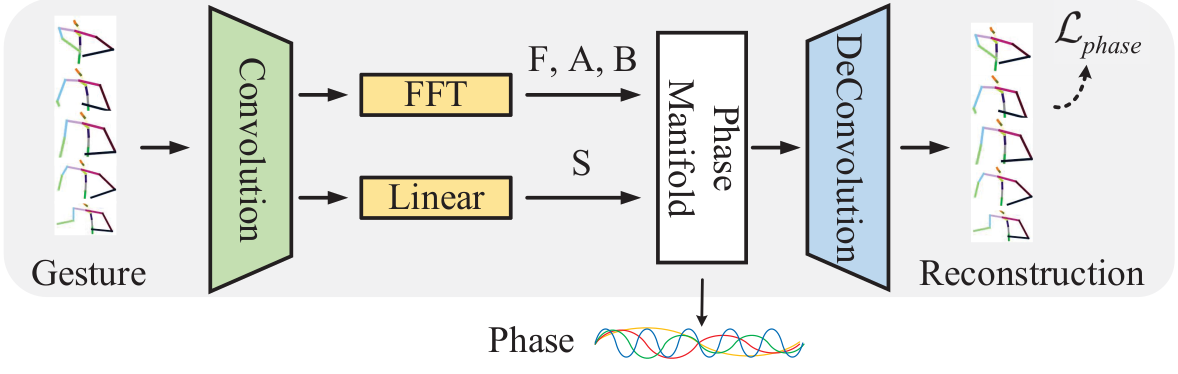
\includegraphics[width=\linewidth]{images/phrase_guidance.png}
%     \caption{Phrase Guidance}
%     \label{fig:PhraseGuidance}
% \end{figure}


% Hàm pha

% $$
% f(\mathcal{T} ; \mathbf{A}, \mathbf{F}, \mathbf{B}, \mathbf{S})=\mathbf{A} \cdot \sin (2 \pi \cdot(\mathbf{F} \cdot \mathcal{T}-\mathrm{S}))+\mathbf{B}
% $$

% Hàm encoder

% $$
% \mathbf{L}=E_{p}(\mathbf{G_{ \text{rotation\_velocity} }})
% $$

% Hàm fourier 
% $$
% \mathbf{c}=F F T(\mathbf{L});\ \ \mathbf{c} \in \mathbb{C}^{M \times K+1}, K=\left|\frac{T}{2}\right|
% $$

% $$
% \mathbf{f}=(0,1 / N, 2 / N, \ldots, K / N)
% $$

% $$
% \mathbf{A}_{i}=\sqrt{\frac{2}{T} \sum_{j=1}^{K} \mathbf{p}_{i, j}}
% $$

% $$
% \quad \mathbf{F}_{i}=\frac{\sum_{j=1}^{K}\left(\mathbf{f}_{j} \cdot \mathbf{p}_{i, j}\right)}{\sum_{j=1}^{K} \mathbf{p}_{i, j}}
% $$


% $$
% \quad \mathbf{B}_{i}=\frac{\mathbf{c}_{i, 0}}{T},
% $$

% Phrase shift
% $$
% \left(s_{x}, s_{y}\right)=F C\left(\mathbf{L}_{i}\right), \quad \mathbf{S}_{i}=\operatorname{atan} 2\left(s_{y}, s_{x}\right)
% $$

% $$
% \mathcal{T}=\left[-\frac{t_{1}-t_{0}}{2},-\frac{t_{1}-t_{0}}{2}+\frac{t_{1}-t_{0}}{N-1}, \ldots, \frac{t_{1}-t_{0}}{2}\right]
% $$


% $$
% \hat{\mathbf{L}}=f(\mathcal{T} ; \mathbf{A}, \mathbf{F}, \mathbf{B}, \mathbf{S})=\mathbf{A} \cdot \sin (2 \pi \cdot(\mathbf{F} \cdot \mathcal{T}-\mathrm{S}))+\mathbf{B}
% $$

% $$
% \hat{\mathbf{G}}_{2}=h(\hat{\mathbf{L}})
% $$

% $$
% \mathcal{P}_{2 i-1}^{(t)}=\mathrm{A}_{i}^{(t)} \cdot \sin \left(2 \pi \cdot \mathrm{S}_{i}^{(t)}\right), \mathcal{P}_{2 i}^{(t)}=\mathrm{A}_{i}^{(t)} \cdot \cos \left(2 \pi \cdot \mathrm{S}_{i}^{(t)}\right)
% $$

% $$
% \mathcal{P} \in \mathbb{R}^{2\ M}
% $$

% $$\mathcal{L}_{\text {phase }}=\mathcal{L}_{\text {phase-recon }}\left(\mathbf{G}, \hat{\mathbf{G}}_{\mathbf{2}}\right)$$




% $$
% \left(
% \left[
%     \hat{
%     \mathcal{P}}_o[-1]^{
%     \left[
%     \left(N_{
%     \text{strid}}-N_{
%     \text{phase}}
% \right):
% \right]}, 
% \mathcal{P}_{a, t}^{
%     \left[N_{
%     \text{strid}}:
% \right]}
% \right]
% \right. 
% , 
% \left.
% \left[
%     \hat{
%     \mathcal{P}}_o[-1]^{
%     \left[-N_{
%     \text{strid}}:
% \right]}, 
% \mathcal{P}_{a, t}^{
%     \left[
%     \left(N_{
%     \text{phase}}-N_{
%     \text{strid}}
% \right):
% \right]}
% \right]
% \right)<
% $$


% $$
% \left(\left[    \hat{    \mathcal{P}}_o[-1]\left[    \left(N_{    \text{strid}}-N_{    \text{phase }}\right):\right], \mathcal{P}_{t, t}^{    \left[        N_{    \text{strid}}:\right]}\right]\right. ,    \left.\left[    \hat{    \mathcal{P}}_o[-1]^{    \left[        -N_{    \text{strid}}:\right]}, \mathcal{P}_{t, t}^{    \left[    \left(N_{    \text{phase }}-N_{    \text{strid}}\right):\right]}\right]\right)
% $$



% $$
% d\left(\operatorname{concat}\left[\hat{\mathcal{P}}_o[-1]\left[\left(N_{\text {strid }}-N_{\text {phase }}\right):\right], \mathcal{P}_{t, t}^{\left[N_{\text {strid }}:\right]}\right]\right. \text {, }   \left.\operatorname{concat}\left[\hat{\mathcal{P}}_o[-1]^{\left[-N_{\text {strid }}:\right]}, \mathcal{P}_{t, t}^{\left[\left(N_{\text {phase }}-N_{\text {strid }}\right):\right]}\right]\right)
% $$

% $$
% d\left(\operatorname{concat}\left[\hat{\mathcal{P}}_o[-1]^{\left[\left(N_{\text {strid }}-N_{\text {phase }}\right):\right]}, \mathcal{P}_{a, t}^{\left[N_{\text {strid }}:\right]}\right]\right. \text {, }   \left.\operatorname{concat}\left[\hat{\mathcal{P}}_o[-1]^{\left[-N_{\text {strid }}:\right]}, \mathcal{P}_{a, t}^{\left[\left(N_{\text {phase }}-N_{\text {strid }}\right):\right]}\right]\right)<
% $$


% $$
% \left[\mathcal{P}_{-1}^{\left[\left(N_{\text {strid }}-N_{\text {phase }}\right):\right]}, \mathcal{P}_{a / t}^{\left[N_{\text {strid }}:\right]}\right]
% $$

% $
% \left[\mathcal{P}_{-1}^{\left[-N_{\text {strid }}:\right]}, \mathcal{P}_{a / t}^{\left[\left(N_{\text {phase }}-N_{\text {strid }}\right):\right]}\right]
% $



